\documentclass{article}
\usepackage[utf8]{inputenc}
\usepackage{latexsym,bm}
\usepackage{mathtools}
\usepackage{amssymb}
\usepackage{cool}
\usepackage{url}
\usepackage[numbers]{natbib}
\usepackage{cleveref}
\usepackage{graphicx}

\newcommand{\defeq}{\mathrel{:\mkern-0.25mu=}}
\newcommand{\eqdef}{\mathrel{=\mkern-0.25mu:}}
\newcommand{\gbinom}{\genfrac[]\z@{}}
\newcommand{\ind}{\perp\!\!\!\!\perp}

\title{The Conditional Bernoulli and its Application to Speech Recognition}
\author{Sean Robertson}

\begin{document}
\maketitle

\section{Motivations} \label{sec:motivations}

A major challenge in speech recognition involves converting a variable number
of speech frames $\{x_t\}_{t \in [1, T]}$ into a variable number of
transcription tokens $\{y_\ell\}_{\ell \in [1, L]}$, where $L \ll T$. In hybrid
architectures, $y_\ell$ are generated as a by-product of transitioning between
states $s_t$ in a weighted finite-state transducer. In end-to-end neural ASR,
this process is commonly achieved either with Connectionist Temporal
Classification (CTC) \cite{gravesConnectionistTemporalClassification2006} or
sequence-to-sequence (seq2seq) architectures
\cite{bahdanauNeuralMachineTranslation2015}. The former introduces a special
blank label; performs a one-to-many mapping $y_\ell \mapsto \tilde{y}_t^{(i)}$
by injecting blank tokens until the transcription matches length $T$ in all
possible configurations $(i)$ during training; and removes all blank labels
during testing. Seq2seq architectures first encode the speech frames $x_t$ into
some encoding $h$, then some separate recurrent neural network conditions on
$h$ to generate the token sequence $y_\ell$.

In 2017, \citeauthor{luoLearningOnlineAlignments2017} developed a novel
end-to-end speech recognizer. Given a prefix of acoustic feature frames
including the current frame $\{x_{t'}\}_{t' \in [t, T]}$ and a prefix of
Bernoulli samples excluding the current frame $\{b_{t'}\}_{t' \in [t+1,T]}$,
the recognizer produces a Bernoulli sample for the current frame $B_t \sim
    P(b_t|x_{\leq t}, b_{<t})$, plus or minus some additional conditioned terms.
Whenever $B_t = 1$, the model ``emits'' a token drawn from a class distribution
conditioned on the same information $Y_t \sim P(y_t|x_{\leq t}, b_{<t})$. The
paper had two primary motivations. First, though it resembles a decoder in a
\textit{seq2seq} architecture \cite{bahdanauNeuralMachineTranslation2015}, it
does not need to encode the entire input sequence $x_t$ before it can start
making decisions about what was said, making it suitable to online recognition.
Second, we can interpret the emission points, or ``highs,'' of the Bernoulli
sequence $B_t = 1$ as a form of hard alignment: the token output according to
$Y_t$ is unaffected by speech $x_{>t}$\footnote{
    %
    This is not necessarily a synchronous alignment. $B_t = 1$ may occur well
    after whatever caused the emission. The last high $\arg\max_{t' < t} B_{t'}
        = 1$ cannot be assumed to bound the event to times after $t'$ for the same
    reason. Finite $t$ and vanishing gradients will force some synchronicity,
    however.
    %
}.

Because of the stochasticity introduced by sampling $B_t$ discretely, the
network cannot determine the exact gradient for parameterizations of $B_t$.
Thus, the authors rely on an estimate of the REINFORCE gradient
\cite{williamsSimpleStatisticalGradientfollowing1992}:
%
\begin{equation} \label{eq:luo_reinforce}
    \pderiv{R}{\theta} = \mathbb{E}_b\left[
    \Sum{\left(\pderiv{R_t}{\theta} +
    \left(\Sum{R_{t'}}{t' \geq t}\right)
    \pderiv{}{\theta}\log P(b_t|b_{<t},y_{<\ell_{t}})
    \right)}{t,1,T}\right]
\end{equation}
%
where
%
\begin{equation} \label{eq:luo_reward}
    R_t = \begin{cases}
        \log P(Y_t = y_{\Sum{b_{t'}}{t' < t}}|
        x_{\leq t}, b_{<t}, y_{\Sum{b_{t'}}{t' < t - 1}})
          & \text{if }B_t = 1 \\
        0 & \text{if }B_t = 0
    \end{cases}
\end{equation}
%
The reward (\cref{eq:luo_reward}) is the log probability of the $k$-th class
label, where $k$ counts the number of high Bernoulli values up to and
including time step $t$. The return for time step $t$ accumulates the
instantaneous rewards for all non-past time steps $t' \geq t$.

In practice, using \cref{eq:luo_reinforce} is very slow to train and yields
mixed results. The authors found it was necessary to add a baseline function
and an entropy function in order to converge. In a later publication
\cite{lawsonLearningHardAlignments2018}, a bidirectional model\footnote{
    %
    Forgoing the motivation for online speech recognition.
    %
} used Variational Inference to speed up convergence, though this failed to
improve the overall performance of the model on the TIMIT corpus. The mixed
performance and convergence of these models was blamed on the high-variance
gradient estimate of \cref{eq:luo_reinforce}
\cite{lawsonLearningHardAlignments2018}.

We believe that the performance and convergence issues of these models are not
due, at least in whole, to a high-variance estimate. Instead, we propose that a
a bias was introduced into \cref{eq:luo_reinforce} via the mechanism which
guaranteed a fixed number of Bernoulli highs during training.

In order to ensure the total number of high Bernoulli values matched the total
number of labels $L$ during training, i.e. $\sum_t b_t = L$, the authors would
force later samples to some specific value. For example, if at point $t = T - L
    + \ell$ only $\ell$ samples emitted, $B_t = 1$ regardless of $P(b_t)$.
Likewise, if $L$ samples emitted before $t$, $B_t = 0$.

% \begin{figure}
%     \centering
%     \begin{minipage}{.45\textwidth}
%         \begin{tabular}{c c c | c}
%             $b_1$ & $b_2$ & $b_3$ & Bias weight \\
%             \hline
%             0 & 0 & 0 & \\[-1.5ex]
%             \hline\noalign{\vspace{\dimexpr 1.5ex-\doublerulesep}}
%             0 & 0 & 1 & $2 \times$ \\
%             0 & 1 & 0 & $2 \times$ \\
%             0 & 1 & 1 & \\[-1.5ex]
%             \hline\noalign{\vspace{\dimexpr 1.5ex-\doublerulesep}}
%             1 & 0 & 0 & $4 \times$ \\
%             1 & 0 & 0 & \\[-1.5ex]
%             \hline\noalign{\vspace{\dimexpr 1.5ex-\doublerulesep}}
%             1 & 0 & 1 & \\[-1.5ex]
%             \hline\noalign{\vspace{\dimexpr 1.5ex-\doublerulesep}}
%             1 & 1 & 1 & \\[-1.5ex]
%             \hline\noalign{\vspace{\dimexpr 1.5ex-\doublerulesep}}
%         \end{tabular}
%     \end{minipage}
%     \begin{minipage}{.45\textwidth}
%         \begin{tabular}{c | c}
%                         & Average $\sum R_t$ \\
%             \hline
%             Unbiased    & $R_1 / 3 + R_2 / 3 + R_3 / 3$ \\
%             Biased      & $R_1 / 2 + R_2 / 4 + R_3 / 4$
%         \end{tabular}
%     \end{minipage}
%     \caption{
%         Example of the effect of sample bias on total reward under a uniform
%         prior.}
%     \label{fig:bias}
% \end{figure}

Though this bias appears harmless at first, it has great ramifications for the
estimator early on during training. We will provide an illustrative example.

Upon initialization of our network, we expect any dependencies between
Bernoulli variables to be negligible. Thus, for the purposes of this example,
we make the strong assumption that they are distributed i.i.d. with probability
$p$. Since the variables are identically distributed, each has an equal
probability of being chosen as one of the $L$ highs, making $P(B_t=1|L) = L /
T$. However, under the reasonable assumptions $0 < L < T - L < T$, the emission
probability for some given $t$ induced by the forced-suffix mechanism evaluates
to
%
\begin{equation} \label{eq:iid_suffix_dist}
    \begin{split}
        P^*(B_t=1|L < T - L < T)
        =& p - I[t > L]p\bar{B}(p; L, t - L) + \\
        &  I[t > T - L](1 - p)\bar{B}(1 - p; T - L; t - T + L)
    \end{split}
\end{equation}
%
Where $I[\ldots]$ is the indicator function and $\bar{B}(p; a, b)$ is the
Regularized Incomplete Beta function. The derivation of this distribution can
be found in \cref{sec:suffix}. The first $t \leq L$ Bernoulli variables
get to ignore the restriction entirely, giving them a probability $p$; the
samples $t > L$ lose out on some of that probability mass because some paths
that would have contributed would have more than $L$ samples; and, samples
$t > L - T$ gain some additional probability mass when they are forced to $1$
in order to emit $L$ highs by the end of the utterance.

\begin{figure}
\centering
\begin{minipage}{0.45\textwidth}
    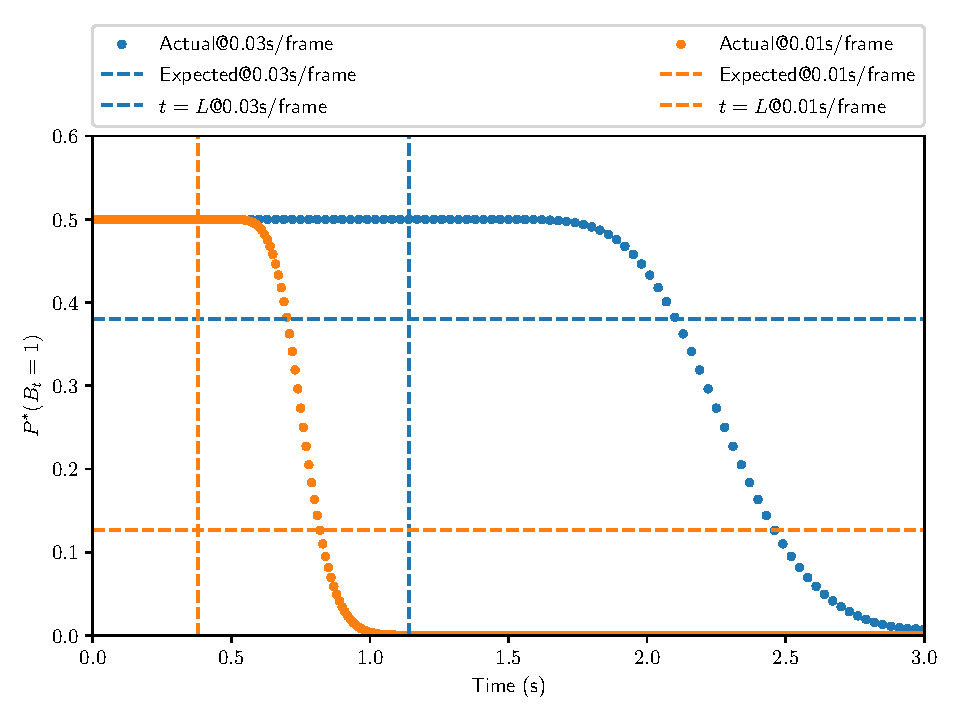
\includegraphics[width=\textwidth]{fs_compare_fs.pdf}
\end{minipage}
\begin{minipage}{0.45\textwidth}
    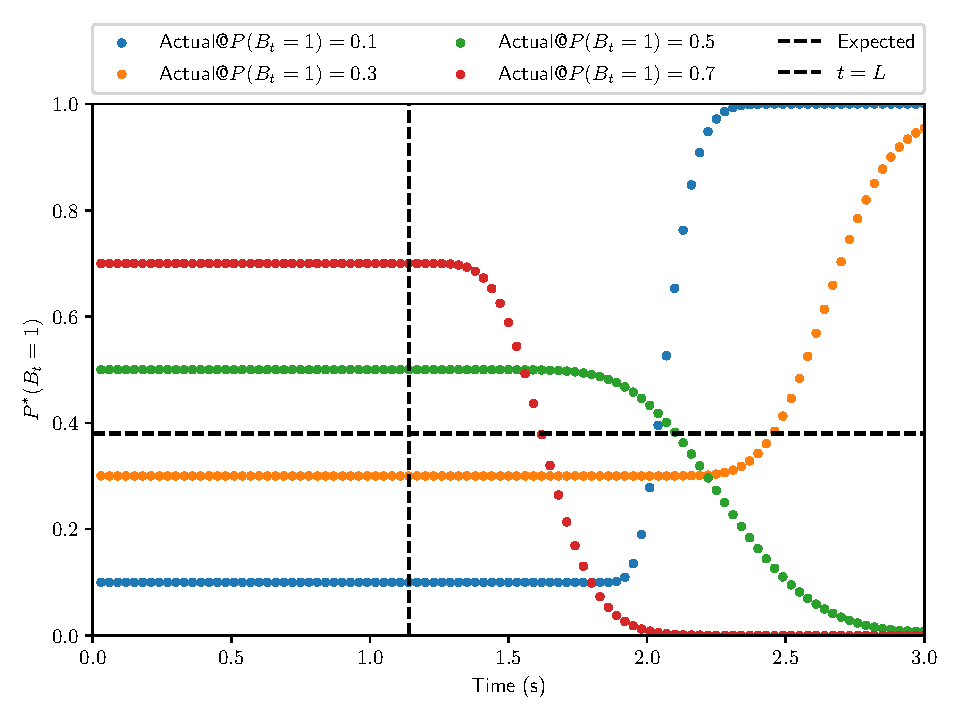
\includegraphics[width=\textwidth]{fs_compare_ps.pdf}
\end{minipage}
\caption{
    %
    The disparity between the expected and actual probabilities of each
    Bernoulli random variable being high over time due to the forced suffix
    hack. Horizontal lines indicate the expected probability for the given
    number of frames and labels. Vertical lines indicate when the frame number
    matches the label number. \emph{Left}: varying frame rate at $p = 0.5$.
    \emph{Right}: varying $p$ at frame rate of $0.03s$.
    %
} \label{fig:bias}
\end{figure}

\Cref{fig:bias} illustrates the distribution of $P^*(B_t=1|\ldots)$ on an
average-length utterance of TIMIT (3 seconds) and an average number of labels
per utterance (38). The blue scatter plot on the left-hand side produces a
Bernoulli random variable every 30 milliseconds, the same as
\citet{luoLearningOnlineAlignments2017}, with even odds of each value. The
forced suffix distribution overestimates the probability of the first two
thirds of samples being and underestimates the last third, with the last sixth
rarely if ever being sampled. The disparity becomes more exaggerated when we
produce a random variable every 10 milliseconds (the orange scatter plot) -
the usual rate at which speech features are produced - with over half of the
Bernoulli variables having virtually zero probability of drawing value $1$. The
right-hand plot illustrates that the bias becomes more or less severe depending
on how close $P(B_t=1)$ is to the expected probability $L / T$.

While \cref{eq:iid_suffix_dist} makes strong independence assumptions about the
Bernoulli random variables, the fundamental flaw with the distribution will
hold even if we relax these assumptions. Even under the distribution with
dependence, a prefix of Bernoulli random variables will ignore the conditioning
on the number of labels, $t \leq L \implies P^*(b_t|b_{<t}, L) =
P(b_t|b_{<t})$, whose over- or underestimation of $P(b_t|b_{<t}, L)$ will be
paid for in the suffix through either under- or overestimation itself. Indeed,
\citet{luoLearningOnlineAlignments2017} observed this predicted behaviour
themselves: without an additional entropy penalty, the model would learn to
emit entirely at either the beginning or end of the sequence.

To solve the problem of bias, we propose replacing the $T$ independent
Bernoulli random variables $B_t$ sampled during training with a single sample
$B$ from the Conditional Bernoulli (CB) distribution during training. The CB
conditions on the required number of high trials, which will make the objective
well-defined during training. It avoids placing undue emphasis on earlier
trials, which should curtail the convergence problems faced by
\citet{luoLearningOnlineAlignments2017}. In addition, the CB can be decomposed
into Bernoulli trials that condition on past trial results, similar to
\cref{eq:luo_reward}. We also show how the CB can be relaxed to a continuous
variable for use in Straight-Through estimators
\cite{bengioEstimatingPropagatingGradients2013,jangCategoricalReparameterizationGumbelSoftmax2017}
or RELAX-like estimators
\cite{maddisonConcreteDistributionContinuous2017,grathwohlBackpropagationVoidOptimizing2018}.
Finally, we outline under which conditions the likelihood of $y$ can be exactly
and efficiently calculated under the assumptions of the CB, and how it relates
to CTC and RNN Transducers \cite{gravesSequenceTransductionRecurrent2012}.

\section{The Conditional Bernoulli} \label{sec:cb}
\subsection{Definitions} \label{sec:cb_defns}

The Conditional Bernoulli distribution
\cite{chenWeightedFinitePopulation1994,chenStatisticalApplicationsPoissonBinomial1997},
sometimes called the Conditional Poisson distribution
\cite{tilleSamplingAlgorithms2006,bondessonParetoSamplingSampford2006},
is defined as
%
\begin{equation} \label{eq:cb}
    P\left(b\middle|\Sum{b_t}{t} = k; w\right) = \frac{\Prod{w_t^{b_t}}{t}}
    {\Sum{\Prod{w_t^{b'_t}}{t}}{\left\{b' : \sum_t b_t' = k\right\}}}
\end{equation}
%
Where $w_t = p_t/(1 - p_t)$ are the odds/weights of a Bernoulli random variable
$B_t \sim P(b_t;w_t) = p_t^{b_t} (1 - p_t)^{(1 - b_t)} = w_t^{b_t}/(1 + w_t)$.
\Cref{eq:cb} reads as ``what is the probability that Bernoulli random variables
$B = \{B_t\}_{t \in [1,T]}$ have values $\{b_t\}_t$, given that exactly $k$ of
them are high ($\Sum{b_t}{t} = k$)?'' Letting $K = \Sum{B_t}{t}$, $K$ is a
random variable that counts the total number of ``highs'' in a series of
Bernoulli trials. $K$ is distributed according to the Poisson-Binomial (PB)
distribution, a generalization of the Binomial distribution for when $p_i \neq
p_j$. It is defined as
%
\begin{equation} \label{eq:pb}
    \begin{split}
        P(K = k;w) & = \Sum{P(b;w)}{\left\{b : \sum_t b_t = k\right\}} \\
        & = \left(\Prod{1 + w_t}{t,1,T}\right)^{-1}
        \Sum{\Prod{w_t^{b_t}}{t,1,T}}{\left\{b : \sum_t b_t = k\right\}}
    \end{split}
\end{equation}
%
If we use \cref{eq:pb} to marginalize out $K$ from \cref{eq:cb}, we recover the
independent Bernoulli probabilities:
%
\begin{equation}
    \begin{split}
        P(b; w) &= \Sum{P(b, k; w)}{k,0,T} = \Sum{P(b|k; w) P(k; w)}{k,0,T} \\
        &= P(b|k'; w) P(k'; w) \text{ for exactly one } k' = \sum_t b_t\\
        &= \left(\Prod{1 + w_t}{t}\right)^{-1}\frac{\Prod{w_t^{b_t}}{t,1,T}}
        {\Sum{\Prod{w_t^{b'_t}}{t,1,T}}{\left\{b' : \sum_t b_t' = k'\right\}}}
        \left(\Sum{\Prod{w_t^{b'_t}}{t,1,T}}{\left\{b' : \sum_t b_t' = k'\right\}}\right) \\
        &= \Prod{(1 + w_t)^{-1} w_t^{b_t}}{t,1,T}
    \end{split}
\end{equation}
%
Which is to say that, if we do not have knowledge of the number of highs
\textit{a priori}, assuming a Poisson-Binomial prior, the probability of
sample $B$ is the product of the probabilities of the outcomes of $T$
independent Bernoulli trials.

Direct calculation of equation \cref{eq:cb} involves summing over
$T$-choose-$k$ products of $k$ odds, making it infeasible for large $T$ and
$k$. To combat this, \citet{chenStatisticalApplicationsPoissonBinomial1997}
propose a number of alternative algorithms where the sample $B$ is constructed
by iteratively deciding on the individual values of $B_i$. We will not only use
these algorithms for efficiency: we will also use them to factor the CB
distribution into useful forms for different objectives.

To better describe these algorithms, we define the set of indices $t \in [1, T]
    = I$ s.t. $B = \{B_t\}_{t \in I}$. The set $A \subseteq I$ maps to some sample
$B$ such that all the high Bernoulli variables' indices can be found in $A$,
i.e. $B_t = 1 \iff t \in A$. Then the CB can be restated as
%
\begin{equation} \label{eq:cb_set}
    P(A|k; w) = \frac{\prod_{a \in A} w_a}{C(k, I; w)}
\end{equation}
%
where
%
\begin{equation} \label{eq:C}
    C(v, S; w) = \Sum{\Prod{w_a}{a \in A'}}{\{A' \subseteq S : |A'| = v\}}
\end{equation}
%
normalizes over all possible $k$-tuples of $w_i$ in some set $S$. \Cref{eq:C}
can be considered a generalization of the binomial coefficient, which can be
recovered by setting all $w_t = 1$. If we identify the product of weights from
a set $A$ as a weight indexed by $A$ (i.e. $\Prod{w_a}{a \in A} \mapsto w'_A$),
we can interpret \cref{eq:cb_set} as a categorical distribution.

The Draft Sampling procedure
\cite{chenStatisticalApplicationsPoissonBinomial1997} recursively builds $A$ by
choosing a new weight to add to an ordered set. We use $j \in [1, T]$ to index
elements of $I$ in the order in which they are drafted into $A$: $I =
    \{t_j\}_j$, $A_j = (t_1, t_2, \ldots t_j)$, and $A^c_j = I \setminus A_j =
    \{t_{j + 1}, t_{j + 2}, \ldots, t_T\}$. Then the probability that some $t \in
    A^c_{j - 1}$ is the $j$-th sample to be drafted into $A$ is defined as
%
\begin{equation} \label{eq:draft}
    P(t \in A_j|A_{j-1}, k; w) =
    \frac{w_t C(k - j, A^c_{j-1} \setminus \{t\}; w)}
    {(k - j + 1) C(k - j + 1, A^c_{j-1}; w)}
\end{equation}
%
Terms in both the numerator and denominator of \cref{eq:draft} sum over suffix
sets of length $k - j + 1$ that could be appended to $A_{j-1}$ to get a
$k$-tuple $A$. The numerator is the sum of products of odds including $w_t$.
The conditional probability is conditioned on the remaining (``future'') odds
with respect to $j$, as well as whatever samples $t_j$ were chosen in the past.
The total probability of a drafted sample is
%
\begin{equation} \label{eq:db}
    \begin{split}
        P(A_k|k; w) &= \Prod{P(t_j \in A_j|A_{j-1}; w)}{j,1,k} \\
        &= \Prod{\frac{
        w_{t_j} C(k - j, A^c_j; w)}{
        (k - j + 1)C(k - j + 1, A^c_{j - 1}; w)}
        }{j,1,k} \\
        &= \left(\Prod{w_{t_j}}{j,1,k}\right)
        \frac{C(0,A^c_k; w)}{\Factorial{k} C(k, I; w)} \\
        &= \frac{1}{\Factorial{k}} P(A|k, w)
    \end{split}
\end{equation}
%
\Cref{eq:db} produces almost the same probability as the Conditional
Bernoulli, except for the factorial term. The factorial term accounts for the
fact that samples are drafted into $A_k$ in some fixed order. Summing over the
probabilities of the $\Factorial{k}$ possible permutations of $A_k$ yields the
Conditional Bernoulli. We will call the distribution defined in \cref{eq:db}
the Draft Bernoulli (DB). Though the DB is not the same distribution as the CB,
an expected value over the DB will be the same as that over the CB as long as
the order of samples in $A_k$ is ignored by the value function.

The ID-Checking Sampling procedure
\cite{chenStatisticalApplicationsPoissonBinomial1997} is another useful
treatment of the CB. This procedure builds $A$ by iterating over Bernoulli
trials and making binary decisions whether to include the trial in $A$. First,
choose and fix an order $j$ in which samples $I$ will potentially be added to
$A$. Let $A_{r_j,j} \subseteq A_j = (t_1, t_2, \ldots, t_j)$ be the subset of
$r_j$ samples ($|A_{r_j, j}| = r_j$) that have been added to $A$. At every step
$j$, we choose to either add $t_j$ to $A_{r_{j-1},j-1}$ and recurse on
$A_{r_j,j} = A_{r_{j-1},j-1} \cup \{t_j\}$ or exclude $t_j$ and recurse on
$A_{r_j, j} = A_{r_{j-1},j-1}$. The probability of including $t_j$ is
%
\begin{equation} \label{eq:id_step}
    P(t_j \in A_{r_j,j}|A_{r_{j-1}, j-1}, k; w) =
    \frac{w_{t_j} C(k - r_{j-1} - 1, A_j^c; w)}
    {C(k - r_{j-1}, A_{j-1}^c; w)}
\end{equation}

From the perspective of Bernoulli trials, $P(t_j \in A_{r_j, j}|\ldots) =
    P(B_{t_j} = 1|k - r_j; w)$. \Cref{eq:id_step} can be interpreted as the
probability that $B_{t_j}$ is high, given that $k - r_j$ remaining trials must
be high. Like in \cref{eq:draft}, the numerator and denominator of
\cref{eq:id_step} consist of products of weights of possible suffixes. The
numerator only includes suffixes where $w_{t_j}$ is a multiplicand.

The joint probability of a prefix of Bernoulli trials
$b_{t_{\leq j}} = (b_{t_1}, b_{t_2}, \ldots, b_{t_j})$ using \cref{eq:id_step}
equals
%
\begin{equation} \label{eq:idb}
    \begin{split}
        P(b_{t_{\leq j}}|k - r_j; w)
        &= \Prod{P(b_{t_{j'}}|k - r_{j'}; w)}{j',1,j} \\
        &= \Prod{
        \frac{w_{t_{j'}}^{b_{t_{j'}}}C(k - r_{j'}, A_{j'}^c; w)}
        {C(k - r_{j' - 1}, A_{j'-1}^c; w)}
        }{j',1,j} \\
        &= \left(\Prod{w_{t_{j'}}^{b_{t_{j'}}}}{j',1,j}\right)
        \frac{C(k - r_j, A^c_{j}; w)}{C(k, I; w)}
    \end{split}
\end{equation}
%
The dependence on prior trials is implicit in the $r_{j'}$ term. We will call
the family of distributions over different prefixes the ID-checking Bernoulli
(IDB). When the prefix is the length of the entire sequence $j = T$,
$P(b_{t_{\leq T}}|k - r_T; w) = P(b| k; w)$ and the IDB distribution matches
the CB distribution.

We will find a novel third decomposition useful. This method combines the
ID-Checking and Drafting methods so that the draft at a given step must come
from a bounded suffix of weights. Define $A_{r, j_r} \subseteq A_{j_r} = (t_1,
    t_2, \ldots t_{j_r})$ to be the $C$ samples of $A_{j_r}$ that have been added
to $A$. Define the probability that the next sample $t_j \in A_{t_{j_{r - 1}}}$
is the $r$-th drafted sample to be
%
\begin{equation} \label{eq:bounded_draft}
    P(j = j_r|k - r, j_{r-1}; w) =
    \frac{w_{t_j}C(k - r, A_{t_j}^c;w)}
    {C(k - r + 1, A_{t_{j_{r-1}}}^c;w)}
\end{equation}

The draft is bound to the suffix $A_{t_{j_{r-1}}}^c = (t_{j_{r-1} + 1},
    t_{j_{r-1} + 2}, \ldots, t_{j_T})$. Further, the draft requires that if $t_j$
is the $r$-th draft, the remaining drafts must come from indexed values
$t_{>j}$. To balance the restriction, earlier $t_j$ will be more probable than
later $t_j$ to be drafted earlier. Using the fact that $C(k - r + 1, A_{t_j}^c;
    w) = w_{t_j + 1} C(k - r, A_{t_j + 1}^c; w) + C(k - r + 1, A_{t_j + 1}^c; w)$,
it is easily shown via induction that $C(k - r + 1, A_{t_{j_{r-1}}}^c; w) =
    \Sum{w_{t_j}C(k - r, A_{t_j}^c;w)}{j,j_{r-1}+1,T}$, proving that
\cref{eq:bounded_draft} is a valid probability distribution. The probability of
a draft prefix is calculated as
%
\begin{equation} \label{eq:bb}
    \begin{split}
        P(A_{r, j_r}|k - r; w)
        &= \Prod{P(j_{r'}|k - r', j_{r'-1}; w)}
        {r',1,r} \\
        &= \Prod{
            \frac{w_{t_{j_{r'}}}C(k - r', A_{t_{j_{r'}}}^c;w)}
            {C(k - r' + 1, A_{t_{j_{r'-1}}}^c;w)}
        }{r',1,r} \\
        &= \left(\Prod{w_{t_{j_{r'}}}}{r',1,r}\right)
        \frac{C(k - r, A_{t_{j_r}}^c; w)}{C(k, I; w)}
    \end{split}
\end{equation}
%
We call this distribution the Bounded Bernoulli (BB). When $r = k$, the BB
matches the CB. The BB fixes the multiple orderings problem of the DB. The
conditional probabilities of \cref{eq:bounded_draft} can be efficiently
calculated using intermediate values when calculating $C$ using Method 2 from
\cite{chenStatisticalApplicationsPoissonBinomial1997}. Observing
\cref{eq:idb,eq:bb}, the probability of a prefix under the IDB matches a
probability of some BB draft prefix whenever the last sampled Bernoulli from
the IDB was high. Assuming $b_{t_j} = 1$ and $\Sum{b_{t_{j'}}}{j',1,j} = r$,
$b_{t_{\leq j}} \mapsto A_{r,j_r}$ by the relation $b_{t'} = 1 \Leftrightarrow
    t' \in A_{r,j_r}$. The BB allows us to marginalize out prior drafted samples
and ask what the probability is that $t_j$ is the $r$-th drafted sample:
%
\begin{equation} \label{eq:bb_margin}
    \begin{split}
        P(j = j_r|k - r; w)
        &= \sum_{A_{r, j_{r - 1}}} P(A_{r, j_r}|k - r; w) \\
        &= \left(
        \sum_{\{j_{< r} : j_{r'} < j\}}
        \Prod{w_{t_{j_{r'}}}}{r',1,r-1}
        \right)
        \frac{w_{t_j}C(k - r, A_{t_j}^c; w)}{C(k, I; w)}  \\
        &= \frac{C(r - 1, A_{t_{j-1}}; w)w_{t_j}C(k - r, A_{t_j}^c; w)}{C(k, I; w)}
    \end{split}
\end{equation}
%
The second line features sums over the possible size-($r-1$) prefixes that
could have been drafted prior to $j$, which means that each occurs within the
subset $A_{t_{j - 1}}$. Intuitively, the numerator enumerates all possible
prefixes and all possible suffixes around $w_{t_j}$, subject to the constraint
that $r - 1$ elements come before and $k - r$ come after.

$t_j$ being the $r$-th drafted sample and $t_j$ being the $(r + 1)$-th drafted
sample are clearly disjoint events. Summing over these disjoint probabilities
recovers the probability that $t_j$ belongs to $A$:
%
\begin{equation}
    \begin{split}
        \Sum{P(j = j_r|k - r; w)}{r,1,k}
        &= \frac{w_{t_j}}{C(k, I; w)}
        \Sum{C(r - 1, A_{t_{j-1}}; w)C(k - r, A_{t_j}^c; w)}{r,1,k} \\
        &= \frac{w_{t_j} C(k - 1, I \setminus \{t_j\})}{C(k, I; w)}
    \end{split}
\end{equation}
%
where the second line follows from noting $A_{t_{j-1}} \cup A_{t_j}^c = I
    \setminus \{t_j\}$ and applying Proposition 1.c. from
\citet{chenWeightedFinitePopulation1994}:
%
\begin{equation} \label{eq:vandermonde_r}
    \forall S \subseteq I \quad C(k, I; w) =
    \Sum{C(r, S; w)C(k - r, I \setminus S; w)}{r,0,k}
\end{equation}
%
a generalization of Vandermonde's identity.

Outside of statistics, \citet{swerskyProbabilisticNchoosekModels2012} linked
the CB distribution with the goal of choosing a subset of $k$ items from a set
of $N$ alternatives. In this case, the $N$ alternatives are class labels, where
one or more class labels may be active at a time. Models could be trained in a
Maximum-Likelihood setting using the CB distribution: $B_n = 1$ implies class
$n$ is present and the probability of the data can be estimated via
\cref{eq:cb}. The authors note that it was insufficient to rely on the implicit
prior induced by training via \cref{eq:cb} and had to explicitly learn and
condition on it.

\citet{xieReparameterizableSubsetSampling2019} approximates the $T$-choose-$k$
sampling procedure by using a top-$k$ procedure called Weighted Reservoir
Sampling. This procedure produces samples in an identical fashion to the
Plackett-Luce (PL) distribution \cite{yellottRelationshipLuceChoice1977}, which
has also been explored in the realm of gradient estimation
\cite{gadetskyLowvarianceBlackboxGradient2020}. While the PL distribution has a
similar construction to the DB, its top-$k$ rankings do not have a uniform
distribution over permutations and, as such, the PL does not match the
expectation of the CB. Nonetheless, estimators involving the DB can be
trivially modified to sample from the PL.

\subsection{REINFORCE Objective} \label{sec:reinforce}

From \cref{sec:motivations}, we are interested in sampling $T$ Bernoulli random
variables such that the total number of emissions/highs matches the number of
tokens $L$ during training. We will start by considering the probability of a
token sequence $y = \{y_\ell\}_{\ell \in [1, L]}$ under a model and work our
way to a REINFORCE objective. For brevity, we supress conditioning on the
acoustic data $\{x_t\}_{t \in [1, T]}$ and model parameters.
%
\begin{equation} \label{eq:breakdown_condition}
    \begin{split}
        P(y)    &= P(y, L) \\
        &= \Sum{P(y, b, L)}{b} \\
        &= \Sum{P(b, L)P(y|b)}{b} \\
        &= P(L)\Sum{P(b|L)P(y|b)}{b|L} \\
        &= P(L)\mathbb{E}_{b|L}\left[P(y|b)\right]
    \end{split}
\end{equation}
%
Where $P(y) = P(y, L)$ follows from the fact that $L$ is a deterministic
function of $y$.

Taking the log, we get
%
\begin{equation*}
    \begin{split}
        \log P(y) &= \log P(L) + \log \mathbb{E}_{b| L}\left[P(y|b)\right] \\
        &\geq \log P(L) + \mathbb{E}_{b| L}\left[\log P(y|b)\right]
    \end{split}
\end{equation*}
%
Where we have used Jensen's Inequality to establish a lower bound. Calling the
bound $R$ and differentiating with respect to some parameter $\theta$, we get
%
\begin{equation} \label{eq:lower_bound}
    \begin{split}
        \pderiv{R}{\theta}  &= \pderiv{\log P(L)}{\theta} + \pderiv{}{\theta}
        \mathbb{E}_{b| L}\left[\log P(y|b)\right]
    \end{split}
\end{equation}
%
We have yet to make any assumptions about the distributions of any $P(\cdot)$,
except to say that $|y| = L$. To recover the REINFORCE objective of
\cref{eq:luo_reinforce}, we assume $B$ is a sequence of independent Bernoulli
trials. Further, we approximate $P(b, L) \approx P(b)$. Then we factor
$P(y, b)$ as \cite{lawsonLearningHardAlignments2018}:
%
\begin{equation} \label{eq:luo_factorization}
    P(y,b) = \Prod{P(y_{\ell_t}|b_{\leq t}, y_{<\ell_t})^{b_t}
    P(b_t|b_{< t}, y_{<\ell_t})}{t,1,T}
\end{equation}
%
where $\ell_t = \Sum{b_t'}{t',1,t}$.

Under these assumptions, the rightmost expectation in \cref{eq:lower_bound}
decomposes into\footnote{
    %
    Thanks to Dieterich Lawson for this derivation.
    %
}
%
\begin{equation*}
    \begin{split}
        \pderiv{}{\theta} \mathbb{E}_{b}\left[\log P(y|b)\right]
        &=  \pderiv{}{\theta} \mathbb{E}_{b}\left[
        \Sum{b_t \log P(y_{\ell_t}|b_{\leq t}, y_{<\ell_t})}
        {t,1,T}\right]\\
        &=  \Sum{\pderiv{}{\theta} \mathbb{E}_{b}\left[R_t\right]}{t,1,T}
        \text{ from \cref{eq:luo_reward}} \\
        &=  \Sum{\pderiv{}{\theta} \mathbb{E}_{b_{\leq t}}
        \left[R_t\right]}{t,1,T}
        \text{ since }R_t\text{ not based on }b_{>t} \\
        &=  \Sum{\mathbb{E}_{b_{\leq t}}\left[
        \pderiv{R_t}{\theta} +
        R_t \pderiv{}{\theta} \log P(b_{\leq t}|y_{<\ell_t})
        \right]}{t,1,T} \\
        &= \Sum{\mathbb{E}_{b_{\leq t}}\left[
        \pderiv{R_t}{\theta} +
        R_t \Sum{
        \pderiv{}{\theta}\log P(b_{t'}|b_{t'-1},y_{<\ell_{t'}})}
        {t' \leq t}
        \right]}{t,1,T} \\
        &= \mathbb{E}_b\left[
        \Sum{\left(\pderiv{R_t}{\theta} +
        \left(\Sum{R_{t'}}{t' \geq t}\right)
        \pderiv{}{\theta}\log P(b_t|b_{<t},y_{<\ell_{t}})
        \right)}{t,1,T}\right]
    \end{split}
\end{equation*}

The expectation of the sum of frame-wise objectives is the same as the
expectation of the ``global'' objective, where no subset of $B$ is attributed
to a given class label $y_\ell$:
%
\begin{equation*}
    \pderiv{}{\theta} \mathbb{E}_b\left[\log P(y|b)\right] =
    \mathbb{E}_{b}\left[
        \Sum{\left(\pderiv{\log P(y_\ell|b)}{\theta} +
            \log P(y_\ell|b) \pderiv{}{\theta}\log P(b)}{\ell,1,L}
        \right)\right]
\end{equation*}
%
However, the frame-wise - or ``local'' - signal is assumed to be less noisy
\cite{mnihNeuralVariationalInference2014}.

The decomposition of $P(y, b)$ from \cref{eq:luo_factorization} is only
well-defined when $|y| = \Sum{b_t}{t,1,T}$. This is not a problem during
testing but it is during training when $|y|$ is fixed. For that reason,
\citet{luoLearningOnlineAlignments2017} hacks the Bernoulli sequence
probabilities using the methods described in \cref{sec:motivations}. This
produces a biased estimator with a variety of problems. If we can condition
the joint on the number of highs in $y$, we can avoid the problem entirely.

The easiest fix to being ill-defined is to remove the auto-regressive property
over Bernoulli trials and treat them as independent: $P(b) =
    \Prod{P(b_t)}{t,1,T}$. In this case, $P(b|L)$ is the CB a global REINFORCE
objective can be defined as
%
\begin{equation} \label{eq:cb_reinforce}
    \pderiv{R}{\theta} = \pderiv{\log P(L)}{\theta} + \mathbb{E}_{b|L}
    \left[
        \pderiv{\Sum{R_t}{t,1,T}}{\theta} +
        \left(\Sum{R_t}{t,1,T}\right)\pderiv{}{\theta}
        \log P(b|L)
        \right]
\end{equation}
%
\Cref{eq:cb_reinforce} is tractable and, unlike \cref{eq:luo_reinforce},
well-defined. Unfortunately, it is no longer autoregressive nor local.

The requirement that the model is not auto-regressive with respect to
sequential $B_t$ is a by-product of sampling from $P(b|L)$. If $P(b|L)$ is a
Conditional Bernoulli, the odds of each Bernoulli trial $w_t$ must be known
before sampling a prefix. In an auto-regressive model, $w_t$ depends on the
prefix of samples. We know of no way to determine all $w_t$ without iterating
through all the sequences of Bernoulli trials with $L$ highs, which would be
intractable. Some distribution other than the CB could be chosen for $P(b|L)$,
but this distribution would need to be able to sample both $P(b_t|b_{< t}, L)$
and $P(b_t|b_{< t})$ (i.e. with or without conditioning on the number of class
labels) without conditioning on the odds of future events. To the best of our
knowledge, existing research meets one, but not both, requirements.

That being said, even though $w_t$ cannot condition on prior samples or class
labels, $R_t = b_t \log P(y_{\ell_t}|\ldots)$ can. The model can still be
auto-regressive, as long as that auto-regression does not impact the odds of a
given Bernoulli sample. We can re-inject the auto-regressive property into the
model by treating $P(y_{\ell_t}|\cdots)$ as the output of an auto-regressive
decoder whose decision to step forward depends on whether $B_t = 1$.

If we still assume no prior dependence between Bernoulli trials $B_t$, the
expectation is over the CB distribution $P(b|L)$. We can use the various
decompositions of the CB defined in \cref{sec:cb_defns} to derive local
gradient estimates.

Our first frame-wise objective is courtesy of the IDB decomposition of the CB
from \cref{eq:idb}. Though a given trial sample $B_{t_j}$ is conditioned on
non-past weights $w_{t_{\geq j}}$, it is only conditioned on samples from the
past $b_{t_{< j}}$. Setting $t_j = j$, we decompose the joint probability of
the class label sequence and the CB sample as
%
\begin{equation} \label{eq:idb_factorization}
    P(y, b|L) = P(y|b,L)P(B|L) =
    \Prod{P(y_{\ell_t}|b_{\leq t},y_{<\ell_t})^{b_t}P(b_t|L - r_t)}{t,1,T}
\end{equation}

\Cref{eq:idb_factorization} is very similar to \cref{eq:luo_factorization},
except the conditioning on the number of class labels $L$ forces $\ell_t$ to
be well-defined whenever $B_t = 1$. The derivation of the IDB REINFORCE
gradient is almost identical to that for \cref{eq:luo_reinforce}, yielding
%
\begin{equation} \label{eq:idb_reinforce}
    \pderiv{R}{\theta} =
    \pderiv{\log P(L)}{\theta} +
    \mathbb{E}_{b|L}\left[
        \Sum{\left(\pderiv{R_t}{\theta} +
            \left(\Sum{R_{t'}}{t' \geq t}\right)
            \pderiv{}{\theta}\log P(b_t|L - \ell_t)
            \right)}{t,1,T}\right]
\end{equation}
%
where $R_t = b_t \log P(y_{\ell_t}|b_{\leq t}, y_{< \ell_t})$.

\Cref{eq:idb_reinforce} is very similar to \cref{eq:luo_reinforce}, but is
unbiased. In the example given in \cref{fig:bias}, the IDB estimate will
treat each valid sequence of Bernoulli trials as equally likely. The sum of
rewards over future trials is a function of the dependence of $R_t$ on past
trials $b_{< t}$.

We can prove that the variance of \cref{eq:idb_reinforce} is no greater than
that of \cref{eq:cb_reinforce}. Representing the expectation in
\cref{eq:idb_reinforce} as $\mathbb{E}_{b|L}[Y]$ and that in
\cref{eq:cb_reinforce} as $\mathbb{E}_{b|L}[Z]$,
%
\begin{equation} \label{eq:cb_idb_equiv}
    \begin{split}
        \mathbb{E}_{b|L}[Z]
        &=  \mathbb{E}_{b|L}\left[
        \pderiv{\Sum{R_t}{t,1,T}}{\theta} +
        \left(\Sum{R_{t'}}{t',1,T}\right)
        \left(\Sum{\pderiv{}{\theta}\log P(b_t|b_{<t}, L)}{t,1,T}\right)
        \right] \\
        &= \mathbb{E}_{b|L}\left[\Sum{\left(
        \pderiv{R_t}{\theta} +
        \left(\Sum{R_{t'}}{t',1,T}\right)
        \pderiv{}{\theta}\log P(b_t|b_{<t}, L)
        \right)}{t,1,T}
        \right] \\
        &= \mathbb{E}_{b|L}\Bigg[\Sum{\left(
        \pderiv{R_t}{\theta} +
        \left(\Sum{R_{t'}}{t',t,T}\right)
        \pderiv{}{\theta}\log P(b_t|b_{<t}, L)
        \right)}{t,1,T} + \\
        &\qquad\qquad
        \Sum{\left(
        \left(\Sum{R_{t'}}{t',1,t-1}\right)
        \pderiv{}{\theta}\log P(b_t|b_{<t}, L)
        \right)}{t,1,T}
        \Bigg] \\
        &= \mathbb{E}_{b|L}[Y + X] \\
        &= \mathbb{E}_{b|L}[Y] + \mathbb{E}_{b|L}[X]
    \end{split}
\end{equation}
%
We can see that $Z = X + Y$. We first prove that the expectation of the
two estimators are equivalent by showing $\mathbb{E}_{b|L}[X] = 0$:
%
\begin{equation} \label{eq:zero_expect_cb}
    \begin{split}
        \mathbb{E}_{b|L}[X] &=
        \mathbb{E}_{b|L}\left[
        \Sum{R_{< t}\pderiv{}{\theta}\log P(b_t|b_{<t}, L - \ell_t)\right]}{t,1,T}\\
        &=  \Sum{\mathbb{E}_{b|L}\left[R_{< t}\pderiv{}{\theta}\log P(b_t|b_{<t}, L - \ell_t)\right]}{t,1,T} \\
        &=  \Sum{\mathbb{E}_{b_{<t}|L}\left[
        \mathbb{E}_{b_t|b_{<t},L}\left[R_{< t}\pderiv{}{\theta}\log P(b_t|b_{<t}, L - \ell_t)\right]
        \right]}{t,1,T} \\
        &=  \Sum{\mathbb{E}_{b_{<t}|L}\left[R_{< t}
        \mathbb{E}_{b_t|b_{<t},L}\left[\pderiv{}{\theta}\log P(b_t|b_{<t}, L - \ell_t)\right]
        \right]}{t,1,T} \\
        &=  \Sum{\mathbb{E}_{b_{<t}|L}\left[R_{< t}
        \pderiv{}{\theta}\mathbb{E}_{b_t|b_{<t},L}[1]
        \right]}{t,1,T} \\
        &= 0
    \end{split}
\end{equation}
%
Now we can treat the random variable $Z$ as a function of $X$ and $Y$,
$Z = X + Y = J(X, Y)$ and calculate the marginal expectation of $Y$:
%
\begin{equation} \label{eq:marginal_expectation}
    \widehat{J}(Y) = \mathbb{E}_x[J(X, Y)|Y] = Y + \mathbb{E}_x[X] = Y
\end{equation}
%
which follows from \cref{eq:zero_expect_cb}. By \cref{eq:cb_idb_equiv},
$\mathbb{E}_y[\widehat{J}(Y)] = \mathbb{E}_y[Y]$ is expectation in the IDB
estimator of \cref{eq:idb_reinforce}. The remainder of the proof is merely an
application of the Rao-Blackwell-Kolmogorov theorem:
%
\begin{equation} \label{eq:rbk}
    \begin{split}
        Var(J(X, Y))
        &= \mathbb{E}_{x,y}[J(X, Y)^2] - \mathbb{E}_{x,y}[J(X, Y)]^2 \\
        &= \mathbb{E}_y[\mathbb{E}_x[J(X, Y)^2|Y]] - \mathbb{E}_{x,y}[J(X, Y)]^2 \\
        &\geq \mathbb{E}_y[\mathbb{E}_x[J(X, Y)|Y]^2] - \mathbb{E}_{x,y}[J(X, Y)]^2 \\
        &= \mathbb{E}_y[\widehat{J}(Y)^2] - \mathbb{E}_{x,y}[J(X, Y)]^2 \\
        &= \mathbb{E}_y[\widehat{J}(Y)^2] - \mathbb{E}_y[\widehat{J}(Y)]^2 \text{ from \cref{eq:cb_idb_equiv}} \\
        &= Var(\widehat{J}(Y))
    \end{split}
\end{equation}
%
where the third line follows from the convexity of $(\cdot)^2$ and Jensen's
Inequality.

The IDB REINFORCE gradient can be more efficiently calculated using the BB
step function. Letting $R_{t_\ell}$ denote the reward for timestep $t_\ell$
whenever $B_t = 1$, all remaining $R_t$ have reward zero. Thus
%
\begin{equation} \label{eq:idb_reinforce_alt}
    \begin{split}
        \pderiv{R}{\theta}
        &=  \pderiv{\log P(L)}{\theta} +
        \pderiv{}{\theta} \mathbb{E}_{b|L}\left[\log P(y|b)\right] \\
        &=  \pderiv{\log P(L)}{\theta} +
        \Sum{\mathbb{E}_{b_{\leq t}|L}\left[
            \pderiv{R_t}{\theta} +
            R_t \pderiv{}{\theta} \log P(b_{\leq t}|L - t_\ell)
            \right]}{t,1,T} \\
        &=  \pderiv{\log P(L)}{\theta} +
        \Sum{\mathbb{E}_{b_{\leq t_\ell}|L}\left[
            \pderiv{R_{t_\ell}}{\theta} +
            R_{t_\ell} \pderiv{}{\theta} \log P(b_{\leq t_\ell}|L - \ell)
            \right]}{\ell,1,L} \\
        &=  \pderiv{\log P(L)}{\theta} +
        \Sum{\mathbb{E}_{t_{\leq \ell}|L}\left[
            \pderiv{R_{t_\ell}}{\theta} +
            R_{t_\ell} \pderiv{}{\theta} \log P(t_{\leq \ell}|L - \ell)
            \right]}{\ell,1,L} \\
        &=  \pderiv{\log P(L)}{\theta} +
        \mathbb{E}_{b|L}\left[
        \Sum{\left(
        \pderiv{R_{t_\ell}}{\theta} +
        \left(\sum_{\ell' \geq \ell}R_{t_{\ell'}}\right)
        \pderiv{}{\theta} \log P(t_\ell|t_{\ell - 1}, L - \ell)
        \right)}{\ell,1,L}
        \right]
    \end{split}
\end{equation}
%
where $R_{t_\ell} = \log P(y_\ell|t_{\leq \ell}, y_{<\ell})$. The
$P(t_\ell|\ldots)$ term is recognized as the BB step function of
\cref{eq:bounded_draft}. \Cref{eq:idb_reinforce_alt} yields identical sample
estimates as \cref{eq:idb_reinforce}, but requires calculation of far fewer
terms.

\Cref{eq:idb_reinforce,eq:idb_reinforce_alt} allow $R_t$ to condition on the
history of Bernoulli trials $b_{< t}$ sampled. For example, $\log
P(y_\ell|t_{\leq \ell}, y_{<\ell})$ can be parameterized by a decoder neural
network which concatenates together a hidden state from an encoder network from
time $t_\ell$ and an embedding of the previous class label $y_{\ell - 1}$ as
input to the RNN. Unfortunately, the dependence on $t_{\leq \ell}$ means that
$t_{\ell'}$ is not only responsible for reward $R_{t_{\ell'}}$, but also for
all rewards succeeding it $R_{t_{\ell' + 1}}, R_{t_{\ell' + 2}}, \ldots$.
For this reason, $\pderiv{}{\theta} \log P(t_\ell|t_{\ell - 1}, L - \ell)$
will tend to receive higher magnitude updates than $t_{\ell + 1}$, which we
expect to increase the variance of the estimator.

We can make the estimator more ``local'' if we make a conditional independence
assumption $P(y_\ell|t_{\leq \ell}, y_{<\ell}) = P(y_\ell|t_\ell, y_{< \ell})$.
This costs us, for example, the ability to feed an encoder hidden state as part
of the input to a decoder RNN since that produces an implicit dependence on all
$t_{\leq \ell}$. Our example decoder may still, however, condition its output
on a hidden state at time $t_{\ell}$ and previous class labels $y_{<\ell}$,
similar to \cite{wuHardNonmonotonicAttention2018}.

Deriving the new estimator is similar to before. Letting $R_{t_\ell} = \log
P(y_\ell|t_\ell,y_{<\ell})$,
%
\begin{equation} \label{eq:bbm_reinforce}
    \begin{split}
        \pderiv{R}{\theta}
        &= \pderiv{\log P(L)}{\theta} +
        \Sum{\pderiv{}{\theta} \mathbb{E}_{b|L}[R_{t_\ell}]}{\ell,1,L} \\
        &= \pderiv{\log P(L)}{\theta} +
        \Sum{\pderiv{}{\theta}
        \mathbb{E}_{t_\ell|L - \ell}[R_{t_\ell}]}{\ell,1,L} \\
        &=  \pderiv{\log P(L)}{\theta} +
        \mathbb{E}_{b|L}\left[
            \Sum{\left(
                \pderiv{R_{t_\ell}}{\theta} +
                R_{t_\ell} \pderiv{}{\theta} \log P(t_\ell|L - \ell)
                \right)}{\ell,1,L}
            \right]
    \end{split}
\end{equation}
%
where $P(t_\ell|L - \ell)$ is the marginal probability of the $t$ being the
$\ell$-th BB-drafted sample, i.e. \cref{eq:bb_margin}. We call this estimator
the Marginal Bounded Bernoulli (MBB) REINFORCE estimator. \Cref{eq:bb_margin}
is similar to \cref{eq:idb_reinforce_alt} but only multiplies the
log-probability of the $t_\ell$-th draft (not all $t_{\leq \ell}$ drafts) with
its local reward $R_{t_\ell}$. This should make the magnitude of the update
more uniform with respect to the timestep.

When we make the conditional independence assumption above, we can prove that
the MBB estimator has variance no greater than that of the IDB estimator.
The proof is similar to that showing the IDB estimator has no greater variance
than that of the CB estimator. First, we split the expectation of the IDB
estimator into two random variables $Z = X + Y$:
%
\begin{equation} \label{eq:idb_bbm_equiv}
    \begin{split}
        \mathbb{E}_{b|L}[Z]
        &= \mathbb{E}_{b|L}\left[
            \Sum{\left(
                \pderiv{R_{t_\ell}}{\theta} +
                R_{t_\ell} \pderiv{}{\theta} \log P(t_{\leq \ell}|L - \ell)
                \right)}{\ell,1,L}\right] \\
        &= \mathbb{E}_{b|L}\Bigg[
            \Sum{\left(
                \pderiv{R_{t_\ell}}{\theta} +
                R_{t_\ell} \pderiv{}{\theta} \log P(t_\ell|L)
                \right)}{\ell,1,L} + \\
            &\qquad\qquad
            \Sum{\left(
                R_{t_\ell} \pderiv{}{\theta}
                \log P(t_{<\ell}|t_\ell,L - \ell)
                \right)}{\ell,1,L}
            \Bigg] \\
        &= \mathbb{E}_{b|L}[Y + X] \\
        &= \mathbb{E}_{b|L}[Y] + \mathbb{E}_{b|L}[X]
    \end{split}
\end{equation}
%
Where we note that the expectation over $Y$ is that of \cref{eq:bbm_reinforce}.
We are left to prove, once again, that $\mathbb{E}_{b|L}[X] = 0$.
%
\begin{equation} \label{eq:zero_exp_idb}
    \begin{split}
        \mathbb{E}_{b|L}[X]
        &= \mathbb{E}_{b|L}\left[
            \Sum{\left(
                R_{t_\ell} \pderiv{}{\theta}
                \log P(t_{<\ell}|t_\ell,L - \ell)
                \right)}{\ell,1,L}
            \right] \\
        &= \Sum{
        \mathbb{E}_{t_{\leq \ell}|L}\left[
            R_{t_\ell} \pderiv{}{\theta}
            \log P(t_{<\ell}|t_\ell,L - \ell)
            \right]}{\ell,1,L} \\
        &=  \Sum{
        \mathbb{E}_{t_\ell|L}\left[
        \mathbb{E}_{t_{<\ell}|t_\ell, L - \ell}\left[
            R_{t_\ell} \pderiv{}{\theta}
            \log P(t_{<\ell}|t_\ell,L - \ell)
            \right]
        \right]}{\ell,1,L} \\
        &= \Sum{
        \mathbb{E}_{t_\ell|L}\left[
        R_{t_\ell} \pderiv{}{\theta}
        \mathbb{E}_{t_{<\ell}|t_\ell, L - \ell}[1]
        \right]}{\ell,1,L} \\
        &= 0
    \end{split}
\end{equation}
%
The remainder of the proof identically follows from
\cref{eq:marginal_expectation,eq:rbk}. We emphasize that this only holds when
$R_\ell$ is memoryless ($R_\ell \ind t_{< \ell} | t_\ell$),. If $R_\ell$ is not
memoryless \cref{eq:bbm_reinforce} is not an unbiased estimator of the total
reward.

Once we have made the conditional independence assumption required for the MBB,
however, we can efficiently calculate the exact expectation using dynamic
programming. We will discuss how in \cref{sec:exact}. The MBB may still be
preferred over the exact form if the cost to compute $R_\ell$ is prohibitively
expensive.

\subsection{Continuous relaxations} \label{sec:relaxations}

A continuous relaxation is a continuous random variable that approximates
(relaxes) some discrete random variable. Of particular note is the
Concrete/Gumbel-SoftMax distribution
\cite{maddisonConcreteDistributionContinuous2017,jangCategoricalReparameterizationGumbelSoftmax2017},
which approximates a categorical random variable $B \in [1, N]$ with odds
$\{w_n\}_{n \in [1, N]}$, Gumbel noise $G_n = -\log(-\log U_n), U_n \sim
    Uniform(0, 1)$, and a scalar temperature $\lambda \in \mathbb{R}^+$. The
Concrete random variable $Z \in \{x \in [0, 1]^N; \Sum{x_n}{n} = 1\}$ is
defined as
%
\begin{equation} \label{eq:concrete}
    Z_n = \frac{\Exp{(\log w_n + G_n)/\lambda}}
    {\Sum{\Exp{(\log w_{n'} + G_{n'})/\lambda}}{n',1,N}}
\end{equation}

A categorical sample $B \sim P(n; N)$ can be recovered from a Concrete sample
in two equivalent manners. First, by the Gumbel-Max trick
\cite{yellottRelationshipLuceChoice1977}:
%
\begin{equation} \label{eq:gumbel_max}
    P(\forall n'. Z_n \geq Z_{n'}) = \frac{w_n}{\Sum{w_{n'}}{n',1,N}} = P(B = n)
\end{equation}
%
Which implies that $B = H(Z) = \arg_n \Max{Z_n}$ is a Categorical sample.
Alternatively, $Z$ approaches a one-hot representation of $B$ as
$\lambda \to 0$:
%
\begin{equation} \label{eq:zero_temperature}
    P(\lim_{\lambda \to 0} Z_n = 1) = \frac{w_n}{\Sum{w_{n'}}{n',1,N}}
    = P(B = n)
\end{equation}

When $N = 2$, $P(B = n)$ is Bernoulli, the Concrete variable is defined as
%
\begin{equation} \label{eq:concrete_bernoulli}
    Z = \frac{1}{1 + \Exp{-(\log w + D)/\lambda}}, D = \log U - \log (1 - U)
\end{equation}
%
and the deterministic mapping $B = H(Z) = I[Z > 0.5]$.

Using the mapping $\Prod{w_a}{a \in A} = w'$, the CB can be considered a
categorical distribution and suitable for a Concrete relaxation. Unfortunately,
using this mapping directly would convert an $N$-length vector of weights $w_n$
to a vector of $N$-choose-$k$ weights, which is intractable for large $N$.
The numerator in \cref{eq:concrete} cannot be teased into a combination of
random variables $W_1(w_1), W_2(w_2), \ldots$, because the Gumbel noise
$G_n$, which would now represent the combination of noise of the $W_a$ terms,
would no longer be independent of $G_{n'}, n' \neq n$. Thus, the CB is not
directly suited to continuous relaxation.

We can, however, relax the CB indirectly by relaxing the intermediate variables
defined in \cref{sec:cb_defns}. The IDB can be relaxed as a sequence of
Bernoulli relaxations of \cref{eq:concrete_bernoulli} according to the
recursive step \cref{eq:id_step}. The BB can be relaxed
into a sequence of categorical relaxations of \cref{eq:concrete} according to
the draft \cref{eq:bounded_draft}. Finally, the marginal probability of
$t_\ell$ under the BB (\cref{eq:bb_margin}) is just one categorical relaxation
per label $\ell$.

When the objective can be reframed in terms of the relaxation $Z$, a network
can start by optimizing a high temperature $\lambda$, then slowly lower it over
the course of training so that $Z$ approaches the discrete distribution. At
test time, the deterministic mapping $H(Z)$ can be used. For our objective, a
relaxed emission does not make sense. We need to come up with $L$
distinct distributions for each of the class labels $y_\ell$.

We focus on two uses of continuous relaxations with a discrete objective. The
first is to use a RELAX-based gradient estimator
\cite{grathwohlBackpropagationVoidOptimizing2018}. RELAX-based gradient
estimators augment the REINFORCE estimator with some additional terms that are
intendent to reduce its variance. Letting $B$ be a discrete random variable of
a continuous relaxation $Z$, the gradient of the expected value of some $f$
(where $f$ can be a reward, e.g.) is defined as
%
\begin{equation} \label{eq:relax}
    \pderiv{\mathbb{E}_b[f(b)]}{\theta} =
    \mathbb{E}_b\left[
        \left(f(b) - \mathbb{E}_{z|b}[\gamma(z)]\right)\pderiv{\log P(b)}{\theta}
        - \pderiv{\mathbb{E}_{z|b}[\gamma(z)]}{\theta}
        \right] + \pderiv{\mathbb{E}_z[\gamma(z)]}{\theta}
\end{equation}
%
Where $\gamma(z)$ is a control variate, e.g. a neural network trained on the
values of the relaxation to minimize the difference between the objective
$f(b)$ and itself. $P(z|b)$ is the truncated distribution over $Z$ such that
the value of $Z$ obeys the relationship $H(Z) = b$. If $\gamma(z)$ is the
concrete distribution parameterized by a learnable $\lambda$, \cref{eq:relax}
is the REBAR gradient \cite{tuckerREBARLowvarianceUnbiased2017}.

RELAX-style estimators can be paired with
\cref{eq:idb_reinforce,eq:bbm_reinforce}. \Cref{eq:idb_reinforce} is preferred
over \cref{eq:idb_reinforce_alt} as the latter would involve infinite values
in the relaxed categorical draft for $t \leq t_{\ell - 1}$. Each Bernoulli in
the IDB format has a real relaxation except when $T - t = L - \ell_t$, at which
point $\log P(b_{\leq t}|\ldots) = 0$ and hence does not need a baseline.
\Cref{eq:bbm_reinforce} is always real.

The second is the so-called Straight-Through (ST) estimator
\cite{bengioEstimatingPropagatingGradients2013,jangCategoricalReparameterizationGumbelSoftmax2017}.
An ST estimator uses the discrete sample $H(X)$ during the forward pass, and
estimates the partial derivative of $H(X)$ in the backward pass with that of
$X$, i.e. $\pderiv{H(X)}{\theta} \approx \pderiv{X}{\theta}$. This estimator is
biased, but can work well in practice. If we output a one-hot representation
$H(X^{(\ell)}) = b^{(\ell)} \in \{0, 1\}^T, b_t^{(\ell)} = 1_{t = n^{(\ell)}}$
for the $\ell$-th drafted (DB or BB) sample, adding them together $b =
    \Sum{b^{(\ell)}}{\ell,1,L}$ produces our CB sample. If we substitute
$\pderiv{b_t^{(\ell)}}{\theta} \approx \pderiv{X_t^{(\ell)}}{\theta}$ then
$\pderiv{b_t}{\theta} = \Sum{\pderiv{b_t^{(\ell)}}{\theta}}{\ell}$ is
well-defined. Alternatively, we can construct $b$ by concatenating together the
relaxed Bernoulli trials of the IDB, $b = [b^{(1)}, b^{(2)}, \ldots, b^{(T)}],
    b^{(t)} = H(X^{(t)})$. Again, the partial derivatives are well-defined:
$\pderiv{b_t}{\theta} = \pderiv{b^{(t)}}{\theta}$. From there, we maximize the
likelihood of the data using the conditional distribution derived from
\cref{eq:luo_factorization}:
%
\begin{equation} \label{eq:st_lik}
    P(y|b, L) = \Prod{P(y_{\ell_t}|h_t, b_{\leq t})^{b_t}}{t,1,T}
\end{equation}
%
where $h_t$ is a hidden state of the network at timestep $t$. Conditioning on
$b_{\leq t}$ is implicit in the definition of $y_{\ell_t}$, though this
conditioning is ignored by the ST estimator.

\subsection{Exact expectations} \label{sec:exact}

Assume $f(b)$ can be decomposed into a product of functions of fixed-length
history ($K$) over event locations $(t_1, t_2, \ldots, t_L)$:
%
\begin{equation} \label{eq:fb_fixed}
    f(b) \defeq \Prod{f_\lambda(\tilde{t}_{\lambda})}{\lambda,1,L}
\end{equation}
%
where we use $\tilde{t}_\lambda \defeq (t_{\max(\lambda - K + 1, 1)},
\ldots, t_\lambda)$ to be the $K$ most recent event locations in $t_{\leq
\lambda}$ (if they exist; otherwise fewer).

Define $\zeta$ as
%
\begin{equation} \label{eq:zeta}
    \zeta(\ell; w, f) \defeq \sum_{t_{\leq \ell}}
        \Prod{w_{t_\lambda} f(\tilde{t}_\lambda)}{\lambda,1,\ell}
\end{equation}

It follows from \cref{eq:fb_fixed,eq:zeta} that
%
\begin{equation}
    \zeta(L; w, f)
        = \sum_{\{ b : \ell_T = L \}} f(b) \Prod{w_t^{b_t}}{t,1,T}
        = R_{train} \Prod{(1 + w_t)}{t,1,T}
\end{equation}
%
which means when $B_t$ are independent and $f(b)$ decomposes into a product of
fixed-history contributions, we can compute our training objective exactly with
$\zeta$.

We can derive a recurrence relation similar to the Howard recurrence by
partitioning $w$. We canonically set $\zeta(0; w, f) = 0$, then
%
\begin{equation} \label{eq:zeta_recurrence}
\begin{split}
    \zeta(\ell; w_{\leq t'}, f) =&
        \left(\sum_{\{t_{\leq \lambda} : t_\lambda < t'\}}
            \Prod{w_{t_\lambda} f(\tilde{t}_\lambda)}{\lambda,1,\ell}\right) +
        \left(\sum_{\{t_{\leq \lambda} : t_\lambda = t'\}}
            \Prod{w_{t_\lambda} f(\tilde{t}_\lambda)}{\lambda,1,\ell}\right) \\
    =&  \zeta(\ell; w_{< t'}, f) +
        \left(\sum_{\{t_{\leq \lambda} : t_\lambda = t'\}}
            \Prod{w_{t_\lambda} f(\tilde{t}_\lambda)}{\lambda,1,\ell}\right)
\end{split}
\end{equation}
%
If $K = 1$, $\tilde{t}_\lambda = (t_\lambda)$ and
%
\begin{equation} \label{eq:zeta_recurrence_k1}
\begin{split}
    \zeta(\ell; w_{\leq t'}, f) =&
            \zeta(\ell; w_{< t'}, f) +
            w_{t'} f_\ell(t') \sum_{\{t_{\ell - 1} : t_{\ell - 1} < t'\}}
                \Prod{w_{t_\lambda} f(\tilde{t}_\lambda)}{\lambda,1,\ell} \\
    =& \zeta(\ell; w_{<t'}, f) +  w_{t'} f_\ell(t') \zeta(\ell - 1; w_{<t'}, f)
\end{split}
\end{equation}

\Cref{eq:zeta_recurrence_k1} is remarkably similar to the Howard recurrence. In
fact, choosing $f(b) \equiv 1$ and $K=1$, \cref{eq:zeta} becomes identical to
\cref{eq:cb}. Therefore, $\zeta$ generalizes $C$ by allowing for ordering
effects.

While we can compute $\zeta$ via recurrence for $K > 1$, the process is more
involved. Unlike in \cref{eq:zeta_recurrence_k1}, we cannot fully separate the
contribution of the next event location because it will depend on some exact,
non-empty prefix of events. To efficiently compute right summand of
\cref{eq:zeta_recurrence}, we introduce an auxiliary function, $\Omega$, over
different near-histories of prefixes $u \defeq (u_i)_{i \in [1, \min(K,\ell)]}$
%
\begin{equation} \label{eq:omega}
\begin{split}
    \Omega(\ell, u; w, f)
    =&
        \sum_{\{t_{\leq \ell} : \tilde{t}_\ell=u\}}
       \Prod{w_{t_\lambda}f_\lambda(\tilde{t}_\lambda)}{\lambda,1,\ell} \\
    =& \begin{dcases}
        w_{u_K}f_\ell(u)
        \Sum{
           \sum_{\{t_{< \ell} : \tilde{t}_{\ell - 1} = u_0 \frown u_{<K}\}}
                \Prod{w_{t_\lambda}f_\lambda(\tilde{t}_\lambda)}{\lambda,1,\ell-1}
        }{u_0,\ell - K,u_1-1} & \ell > K \\
        \Prod{w_{u_i}f_i(u_{\leq i})}{i,1,\ell} & \ell \leq K
        \end{dcases} \\
    =& \begin{dcases}
        w_{u_K}f_\ell(u)
        \Sum{\Omega(\ell - 1, u_0 \frown u_{<K})}{u_0,\ell - K,u_1-1} & \ell > K \\
        w_{u_K}f_\ell(u) \Omega(\ell - 1, u_{<\ell}; w, f) & \ell \leq K
        \end{dcases} \\
\end{split}
\end{equation}
%
Which is to say that the sum of contributions of events sequences of length
$\ell$ and ending in event locations $u$ is the sum of $(\ell - 1)$-length
paths ending in the largest strict prefix of $u$, $u_{<K}$, times the
contribution of $u_K$. In order to sum the contributions of paths ending in the
largest strict prefix, we prepend $u_{<K}$ with any $u_0$ less than $u_1$, the
least element of $u$, and sum over all such $u_0$. When $u = t_{\leq \ell}$,
there is only one path corresponding to the largest strict prefix, $u_{< \ell}
= t_{< \ell}$.

Since the suffixes of sequences of event locations can be used to partition all
event sequences of some fixed length ($t_{\leq \ell} \sim t'_{\leq \ell} \iff
\tilde{t}_\ell = \tilde{t'}_\ell$) and $\Omega$ for that fixed length only sums
over sequences in one partition, $\zeta(\ell; w, f) = \Sum{\Omega(\ell, u; w,
f)}{u}$.

% At the end of \cref{sec:reinforce}, we mentioned that we can marginalize out
% the Bernoulli latent variables efficiently, assuming $P(y_\ell|t_{\leq \ell},
% y_{< \ell}) = P(y_\ell|t_\ell, y_{< \ell})$. Further, it must be feasible to
% calculate that probability for all permutations of $t$ and $\ell$. In the case
% of the model proposed by \cite{luoLearningOnlineAlignments2017}, the
% distribution $\log P(y_t|t_\ell)$ is calculated by a simple linear
% transformation of the RNN hidden state $h_t$ followed by a SoftMax. These
% calculations can be parallelized across $t$ and are fully differentiable. The
% decoder structure of \cite{wuHardNonmonotonicAttention2018} is also a candidate
% as the distribution $P(y_\ell|t_\ell, y_{<\ell})$ is a simple two-layer
% feed-forward neural network on the combination of an encoder and a decoder
% hidden state.

% Starting from \cref{eq:breakdown_condition} and making the conditional
% independence assumption between $t_\ell$ and $t_{\ell - 1}$, we manipulate
% $P(y)$ into a form suitable for dynamic programming.
% %
% \begin{equation} \label{eq:marginalization}
%     \begin{split}
%         P(y) &= P(L)\Sum{P(b|L)P(y|b)}{b} \\
%         &= P(L)\Sum{P(b|L)}{b}\Prod{P(y_\ell|b, y_{<\ell})}{\ell,1,L} \\
%         &= P(L)\sum_{\{t_1, t_2, \ldots, t_\ell\}}
%         P(t_1, t_2, \ldots, t_\ell|L)
%         \Prod{P(y_\ell|t_\ell, y_{<\ell})}{\ell,1,L} \\
%         &= P(L)\Sum{
%         \Sum{P(t_\ell|t_{\ell - 1}, L - \ell)
%         P(y_\ell|t_\ell, y_{<\ell})}
%         {t_\ell,t_{\ell - 1} + 1,T - L + \ell}
%         }{\ell,1,L} \\
%         &= P(L)\Sum{
%         \Sum{P(t_\ell|t_{\ell - 1}, L - \ell)P(y_\ell|t_\ell, y_{<\ell})}
%         {t_\ell,1,T}
%         }{\ell,1,L}
%     \end{split}
% \end{equation}
% %
% where the last line follows as $P(t_\ell|t_{\ell - 1}, L - \ell) = 0$ when
% $t_\ell \leq t_{\ell - 1}$.

% Treating $P(t_\ell|t_{\ell - 1}, L)$ as the transition probability between
% states $t \in [1, T]$ and $P(y_\ell|t_\ell, y_{<\ell})$ as the emission
% probability, \cref{eq:marginalization} can be considered a Hidden Markov Model.
% Thus, $P(y)$ can be efficiently calculated using the forward algorithm. The
% backward step is implicit in the calculation of $P(t_\ell|\ldots)$, which
% effectively marginalizes over all suffixes.

% There exists a relationship between \cref{eq:marginalization} and the CTC
% objective \cite{gravesConnectionistTemporalClassification2006} when the history
% of class labels $y_{< \ell}$ is conditionally independent of the current class
% label $P(y_\ell|t_\ell, y_{< \ell}) = P(y_\ell|t_\ell)$. Recalling that
% $P(L)P(b|L) = P(b)$, the independent Bernoulli probabilities, then define a new
% distribution over an augmented class label set $\{y_t'\} = \{y_t\} \cup \{\_\}$
% as
% %
% \begin{equation} \label{eq:augmented_class}
%     P(y'_t) = \begin{cases}
%         P(B_t = 0)         & y'_t = \_        \\
%         P(B_t = 1)P(y_t|t) & \text{otherwise}
%     \end{cases}
% \end{equation}
% %
% where the label ``\_'' acts as a stand-in for choosing not to emit at a given
% time step. Letting $\beta(y')$ remove all the ``\_'' labels from the augmented
% label set,
% %
% \begin{equation} \label{eq:ctc_obj}
%     \begin{split}
%         P(y) &= \Sum{\Sum{P(b_t)P(y_{\ell_t}|t)^{b_t}}{t,1,T}}{b} \\
%         &= \sum_{\{c': |c| = T \land \beta(y') = c\}}\Sum{P(y'_t|t)}{t,1,T}
%     \end{split}
% \end{equation}
% %
% This expression of the data likelihood is almost identical to that of CTC
% \cite{gravesConnectionistTemporalClassification2006}, with two restrictions.
% First, it assumes the distribution over labels factors as described in
% \cref{eq:augmented_class}. In general, \cref{eq:augmented_class} will lead
% to different gradient updates than directly parameterizing the augmented
% vocabulary $P(y'_t)$ since the blank label has its own parameterization.
% Second, $\beta(y')$ in \cref{eq:ctc_obj} does not reduce repeated labels in
% $c'$\footnote{
%     %
%     To the best of our knowledge, there has been no attempt to explore whether
%     the reduction operation leads to any performance benefits over just using
%     the blank label. \citet{gravesConnectionistTemporalClassification2012}
%     mention that reducing repeated labels existed prior to the blank label in
%     the formation of the CTC objective.
%     %
% }. Assuming it allows for the non-standard adjustment to $\beta$, the data
% likelihood marginalized over latent Bernoulli sequences can be trivially
% implemented using an existing CTC loss function. The additional dependency on
% $y_{< \ell}$ can be considered a generalization of the CTC loss function.

% \begin{figure}
%     \centering
%     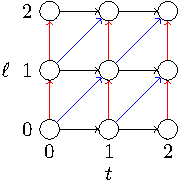
\includegraphics[width=.5\textwidth]{rnnt_vs_cb.pdf}
%     \caption{
%         %
%         A comparison between RNN-T and \cref{eq:marginalization} forward passes
%         over time ($t$) and labels ($\ell$). The RNN-T steps forward in $t$ or
%         $\ell$ independently (black and red lines), while the CB steps forward
%         in either $t$ alone or $t$ and $\ell$ simultaneously (black and blue
%         lines).
%         %
%     } \label{fig:rnnt_vs_cb}
% \end{figure}

% \Cref{eq:marginalization} is similar to the RNN Transducer
% \cite{gravesSequenceTransductionRecurrent2012} with one key difference: the
% RNN-T emits labels and absorbs frames in time separately. \Cref{fig:rnnt_vs_cb}
% illustrates the difference between the two methods' forward calculations. To
% calculate the probability of having emitted the prefix $y_{\leq \ell}$ by time
% $t$, the RNN-T sums contributions from either having seen the entire prefix by
% time $t - 1$ and transitioning to time $t$ via a blank label, or having seen
% $\ell - 1$ labels by time $t$ and then emitting $y_\ell$ (without moving
% forward in time). \Cref{eq:marginalization} maintains the first contribution
% (transitioning from time $t-1$ to $t$ via an implied blank label), but replaces
% the latter with a transition that both absorbs a step in time ($t - 1 \to t$)
% and emits a label ($\ell - 1 \to \ell$).

% The choice to absorb time steps and emit labels independently in the RNN-T
% architecture was motivated partly by the desire to allow sequence transduction
% between inputs and outputs of arbitrary length. \Cref{eq:marginalization}
% requires $L \leq T$, making it (in its current form) unsuited to tasks where
% the output is potentially longer than the input, such as machine translation.
% However, this extra flexibility comes at the cost of uncoupling the events from
% time. Conceptually, the RNN-T models label events as instantaneous, making the
% path where all labels are output at time $t=0$ \textit{a priori} equally likely
% to the path where labels are distributed over time. This has a number of
% practical ramifications. First, when the problem can be conceptualized as
% sequential events in time, the RNN-T wastes probability mass on these
% impossible, instantaneous paths. Second, the monotonicity over $t$ makes
% heuristic search strategies for approximating $\arg_y \max P(y)$ more efficient
% and possibly more accurate for \cref{eq:marginalization} than for
% RNN-Ts\footnote{
% %
%     Such searches, most popularly beam search, involve iteratively building
%     prefix paths over time, pruning low-probability paths. The monotonicity
%     w.r.t. $t$ of \cref{eq:marginalization} ensures only $V + 1$ possible
%     extensions of each stored prefix for the next time step, where $V$ is the
%     size of the vocabulary. Because the RNN-T can output as many labels as it
%     wants at a given time, the search space per prefix is technically
%     arbitrarily big, though practically bounded to some constant positive
%     multiple of $V + 1$.
% %
% }. Finally, \cref{eq:marginalization} can be easily parallelized over labels
% $\ell$ resulting in $O(T)$ serial operations, a na\"{i}ve implementation of the
% RNN-T forward pass requires $O(TL)$ serial operations and a vector-skewed
% implementation requires $O(T + L)$ serial operations
% \cite{bagbyEfficientImplementationRecurrent18}.

% % To prove arbitrarily wide, all you need is T=1. Pick any constant K you'd
% % like, then pick some label set v \in V^K, then make
% % P(blank|v',t=0) = I[v' = v]

% There are two notable extensions that can be made to \cref{eq:marginalization}
% that derive from it being a first-order Markov model. First, we can perform an
% efficient search for $b* = \arg_b \max P(b|y)$ via the Viterbi algorithm. Such
% a search would be performed after training in order to determine the most
% likely times $t* = \{t: b^*_t = 1\}$ when events $y$ occurred in a given window
% of time. Second, we can easily adapt \cref{eq:marginalization} for higher-order
% models so that $P(y_\ell|\ldots)$ can depend on some arbitrary fixed-length
% history of emission points $t_\ell,\ldots,t_{\ell - W + 1}$. While the number
% of states that must be stored for a given order grows exponentially with that
% order, even second-order models may be sufficient to avoid the pitfalls of
% conditionally independent $B_t$. We discuss this more in \cref{sec:approx}.

% Thus, \cref{eq:marginalization} can be
% considered a generalization of CTC.  Finally, the
% estimators from \cref{sec:cb} can also be used as single- or multi-sample
% approximations for CTC.

\section{Approximations} \label{sec:approx}

\begin{figure}
\centering
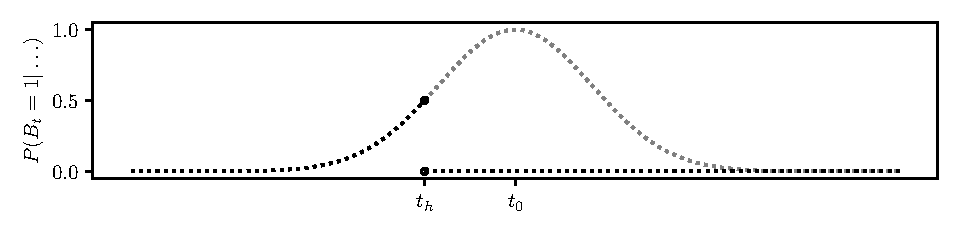
\includegraphics[width=\textwidth]{pro_ar.pdf}
\caption{
%
An example of the different distributions of Bernoulli r.v.s $B_t$ around some
event that occurred at approximately time $t_0$, depending on whether
$P(B_t|\ldots)$ is conditioned on prior $b_{<t}$ (black) or not (grey). $t_h$
is assumed to be a point where both distributions emit $B_{t_h} = 1$.
%
} \label{fig:pro_ar}
\end{figure}

The CB and PB abandon the auto-regressive property of the distribution over
Bernoulli trials. This implies each trial is independent though not necessarily
identically distributed. In this section, we focus on the case of arbitrary
dependencies on past Bernoulli values.

Before continuing, it is worth considering what the auto-regressive property
purchases. Auto-regressive models are often employed in contexts where the
dependent variables are not latent but observable, such as in language
modelling or machine translation. As such, prior claims of the superior
performance of data-conditioned models may not translate to latent-conditioned
models. Also, auto-regressive networks inhibit parallelization during
inference: computations at time $t$ cannot proceed before those at time $t-1$
are completely finished. We can, however, imagine situations where the
additional dependencies would be beneficial. For example, \cref{fig:pro_ar}
illustrates a situation where we are approximating $P(y) \approx P(b, y)$ with
some best-path heuristic at test time. Here we assume some event has occurred
around time $t_0$ but neither a model that parameterizes independent $B_t$
(grey curve) nor a model with dependent $B_t$ (black curves) can localize it to
a specific time. However, after the first high emission at around $t_h$, only
the auto-regressive model can adjust the probability of future $B_t$ to avoid
repeating emissions for the same event. That said, this specific example can be
handled without resorting to arbitrary-length dependencies. We may, for
example, establish a second-order Markov relationship between $y_\ell$ and
$t_\ell$, i.e. $P(y_\ell|t_{\leq \ell}, y_{<\ell}) = P(y_\ell|t_\ell,
t_{\ell-1}, y_{<\ell})$, which can easily penalize emissions that are too
nearby. Qualifiers notwithstanding, we assume for the rest of this section that
an auto-regressive conditional with arbitrarily long history is indeed
worthwhile.

We assume $P(b_t|b_{<t})$ to be well-defined and easily calculable, such as the
output of a recurrent neural network. The general probability over the number
of emissions, $P(L)$, resembles the CB with additional conditional dependence
requirements:
%
\begin{equation} \label{eq:general_pL}
    P(L|b_{<t}) = \sum_{b : \sum_t b_{t'} = L}
    \left( \Prod{P(b_{t'}|b_{<t'})}{t',t,T} \right)
\end{equation}
%
where we have allowed conditioning on an arbitrary prefix of Bernoulli trials
$b_{<t}$ that do not contribute to the count but can change the conditional
probabilities per trial. Making the independence assumption over trials
$P(b_t|b_{<t}) = P(b_t) = \frac{w_t}{1 + w_t}$ recovers \cref{eq:cb}.

We can also express the conditional probability mass function of the next
Bernoulli trial given the remaining number of highs in terms of the
unconditioned probabilities and the distribution over the number of highs:
%
\begin{equation} \label{eq:general_pBgL}
    \begin{split}
        P(b_t|b_{<t}, L)
        &= \frac{P(b_t, L|b_{<t})}{P(L|b_{<t})} \\
        &= \frac{P(b_t|b_{<t})P(L - \Sum{b_{t'}}{t',1,t}|b_{\leq t})}
        {P(L - \Sum{b_{t'}}{t',1,t-1}|b_{<t})}
    \end{split}
\end{equation}

If we consider $P(\ell|\ldots)$ a normalized, conditional version of the count
function $C(\ell, \ldots)$, we can see how an independence assumption would
make \cref{eq:general_pBgL} equivalent to the step distribution of the IDB
\cref{eq:id_step}.

If $P(b_t|b_{<t})$ is unique for the given prefix $b_{<t}$, direct calculations
of \cref{eq:general_pL,eq:general_pBgL} are infeasible given the sheer number
of paths yielding $L$ emissions ($T$ choose $L$). To work around this, we have
to simplify or approximate either $P(b_t|b_{<t})$ or $P(\ell|\ldots)$. The
independence assumption applied is an example of simplifying $P(b_t|b_{<t})$.

This section concerns itself with finding suitable approximations for
\cref{eq:general_pL,eq:general_pBgL}. Specifically, we are interested in
finding a parameterized family of functions $f(b_{<t}, p_{\leq t}, T, L)$ to
approximate $P(B_t=1|b_{<t}, L)$ and one for the prior $P(L)$ via function
family $g(p, T, L)$. The family $f$ only has access to the prefix of samples
$b_{<t}$ and some version of those probabilities $p_{\leq t}$ s.t. $p_t =
    P(B_t=1|b_{<t})$. $f$ does not have access to future $p_t$ in order to allow
for auto-regressive generation of the sample. We assume $p_t \in (0, 1)$ as
most neural networks will parameterize $p_t$ using log-odds\footnote{
    %
    In addition, the only family of approximators that ensure only
    valid $b$ could be sampled is a degenerate one that outputs $B_t = 1$
    whenever $p_t > 1$ and $\sum b_{<t} < L$.
    %
}.

Since we plan on using $f$ to sample a value for $B_t$, it is important that
$f$ only be able to sample values that could be taken by $B_t$ under the
distribution $P(B_t=1|b_{<t}, L)$. Critically, we require that $f$ follow the
restriction that only $L$ high samples may be generated total per sequence.
Formally, letting $\ell_{t-1} = \Sum{b_{t'}}{t',1,t - 1}$, these restrictions
can be stated as
%
\begin{enumerate}
    \item $f(b_{<t}, p_{\leq t}, T, L) = 1$ if $T - t + 1 = L - \ell_{t-1}$.
    \item $f(b_{<t}, p_{\leq t}, T, L) = 0$ if $L - \ell_{t-1} = 0$.
\end{enumerate}
%
that is, the probability of sampling $B_t = 1$ becomes $1$ when the number of
remaining random variables equals the remaining number of highs and becomes
$0$ when all $L$ highs have already occurred.

In what follows, we discuss an additional restriction that would produce an
``ideal'' estimator, then discuss some approximators that we can use instead.

\subsection{The ideal approximation} \label{sec:ideal}

Restrictions 1 and 2 are necessary in order to ensure $f$ produces only
valid samples under the distribution $P(B_t=1|b_{<t}, L)$. This ensures that
$P(y|b)$ is well-defined. This section concerns itself with what additional
restrictions on $f$ and $g$ would be helpful in modelling $P(b|L)$ and $P(L)$.

Restrictions 1 and 2 ensure that the sequence of values $b$ drawn from $f$ are
in the domain of $P(b|L)$, but do not ensure that all valid samples from the
domain of $P(b|L)$ can be drawn. For convenience, define
%
\begin{equation}
    f^{b_t}(b_{<t}, p_{\leq t}, T, L) = \begin{cases}
        f(b_{<t}, p_{\leq t}, T, L)     & b_t = 1 \\
        1 - f(b_{<t}, p_{\leq t}, T, L) & b_t = 0
    \end{cases}
\end{equation}
%
The following restriction ensures the domains of $f$ and $g$ are nonzero
for all nonzero $b$ of $P(b|L)$ and $P(L)$ resp.
%
\begin{enumerate}
    \setcounter{enumi}{2}
    \item $P(L) > 0 \land P(b|L) > 0 \implies
              g(p, T, L) > 0 \land
              \Prod{f^{b_t}(b_{<t}, p_{\leq t}, T, L)}{t,1,T} > 0$
\end{enumerate}
%
Without \emph{a priori} reason for excluding certain samples from the domain
of $f$, not enforcing this restriction would produce situations in inference
where the behaviour of $P(B_t)$ is undefined.

While it is necessary to sample from $P(b|L)$ in order to sample $b$ with
exclusively $L$ highs, we ultimately only care about matching $P(b)$ at test
time. Instead of requiring $P(L) = g(p, T, L)$ and $P(B_t=1|b_{<t}, L) =
f(b_{<t}, p_{\leq t}, T, L)$, $g$ and $p$ could be some other prior and
conditional such that their product is $P(b)$. Formally
%
\begin{enumerate}
    \setcounter{enumi}{3}
    \item $g(p, T, L) = g' > 0 \land
              \Prod{f^{b_t}(b_{<t}, p_{\leq t}, T, L)}{t,1,T} = f' > 0 \implies
              f' g' = P(b)$
\end{enumerate}
%
With restrictions 1-4 we could, for example, derive an unbiased estimator for
$P(y)$ with samples over $f$ and corrected by $g$ in a form similar to
\cref{eq:idb_reinforce}.

The distribution over $b$ induced by the forced-suffix mechanism from
\cref{sec:motivations} is an example of an approximator which satisfies
restrictions 1-3. If we make $f$ only assign one $b$ a nonzero probability and
set $g' = P(b)$, we can satisfy restrictions 1, 2, and 4. However, restrictions
1-4 cannot be met simultaneously. We prove this by counterexample. Choose $T =
2$ and $L = 1$. Note that $B_1 = 1 \iff B_2 = 0$. This means $f(b_1, p_{\leq
2}, 2, 1) = I[b_1 = 0]$ by restrictions 1-2. Let $f(\emptyset, p_1, 2, 1) =
\alpha$. $B_1 = 1$ with probability $\alpha$. Plugging in the samples $b \in
\{0, 1\}^2$ into restriction 3 gives us a system of two equations with two
unknowns ($\alpha$ and $h(\cdot)$):
%
\begin{equation*}
    \begin{split}
        g(p, 2, 1)\alpha &= p_1 (1 - p_2) \\
        g(p, 2, 1)(1 - \alpha) &= (1 - p_1) p_2
    \end{split}
\end{equation*}
%
The system has unique solutions
%
\begin{equation*}
    \begin{split}
        \alpha      &= \frac{p_1 - p_1 p_2}{p_1 - 2 p_1 p_2 + p_2} \\
        g(p, 2, 1)  &= p_1 - 2 p_1 p_2 + p_3
    \end{split}
\end{equation*}
%
which are both valid probabilities. However, the solution to $\alpha$ is a
function of $p_2$, which is not an input to $f(\emptyset, p_1, 2, 1)$. $\alpha$
must be constant for $p = (p_1, p_2)$ and $p' = (p_1, p'_2)$, $p_2 \neq p'_2$,
which means it will not satisfy restriction 4 for all choices of $p$.

This implies there are no $f$ and $g$ that can be decomposed nicely into
$P(b|L)$ and $P(L)$ respectively. In the above counterexample, $p_2$ and $p'_2$
represent the marginal probabilities of the second Bernoulli trial across two
different distributions $p$ and $p'$; they are not conditioned on $b_1$. Thus
we cannot make the decomposition even with the independence assumption, i.e.
$P(b_t|b_{<t}) = P(b_t)$.

Given that 1-4 cannot be satisfied simultaneously, and 1-2 are necessary, we
must decide whether to drop restriction 3 or 4. We believe that it is more
important that the behaviour of our optimized distribution $P(b)$ at test time
be well-defined (though biased) than it is to be unbiased for some choices of
$b$ but undefined for others. While we will present a workaround for
restriction 4, the same trade-off will resurface shortly.

While no $g$ can act as a proper prior $P(L)$, we can still recover the
unconditioned probability of a sample $b$ by relaxing the constraints on $g$.
In particular, if we allow $g$ to depend on the sample $b$, finding $g$ to
satisfy the analogue to restriction 4 is trivial:
%
\begin{equation} \label{eq:g}
    g(b, p, T) = P(b) / \Prod{f^{b_t}(b_{<t}, p_{\leq t}, T, L)}{t,1,T}
\end{equation}
%
from which, if we move the ``prior'' into the expectation, we get
%
\begin{equation} \label{eq:unbiased_approx}
    P(y) = \mathbb{E}_{b \sim f}\left[g(b, p, T)P(y|b)\right]
\end{equation}
%
which can be considered importance sampling
\cite{burdaImportanceWeightedAutoencoders2016}.

While \cref{eq:unbiased_approx} is unbiased, it is high variance and its
gradients suffer from numerical underflow. Instead, we take the log and use
Jensen's Inequality:
%
\begin{equation} \label{eq:vi_lower_bound}
\begin{split}
    \log P(y)
    &= \log \mathbb{E}_{b \sim f}\left[g(b, p, T)P(y|b)\right] \\
    &\geq \mathbb{E}_{b \sim Q}\left[\log \frac{P(y, b)}{Q(b)}\right] \\
    &= \mathbb{E}_{b \sim Q}\left[
        \log P(y) + \log \frac{P(b|y)}{Q(b)}\right]  \\
    &=\log P(y) - \mathcal{D}(Q \| P)
\end{split}
\end{equation}
%
where we have applied \cref{eq:g} and defined $Q(b) = \Prod{f^{b_t}(b_{<t},
p_{\leq t}, T, L)}{t,1,T}$ as the proposal distribution. $\mathcal{D}(Q\|P)$ is
the KL-divergence from $P(b|y)$ to $Q(b)$. This is the same lower bound used in
Variational Inference (VI). Since both $P(b)$ and $Q(b)$ factor over time, we
can apply a similar REINFORCE estimator to \cref{eq:idb_reinforce} and that in
\citet{lawsonLearningHardAlignments2018}, but with the additional restrictions
1-3 on $Q(b)$. The VI lower bound of \cref{eq:vi_lower_bound} hopefully
simultaneously maximizes $P(y|b)$ and forces $Q(b) \to P(b|y)$.

If we consider the right-hand side of \cref{eq:vi_lower_bound} an estimator for
$\log P(y)$, we can see that the estimator is biased unless both sides are
equal. This can only occur when the KL-divergence between $Q(b)$ and $P(b|y)$
is zero. This optimal state cannot be reached in general. This fact follows
almost immediately from the above proof. Choose $P(y|b) = I[\sum_t b_t = L]
P(y)$ which results in $P(b|y) = I[\sum_t b_t = L] P(b)$. Allowing $\sum_t b_t
= L$ and taking $g \equiv 1$ in the above proof, we have already shown $Q(b)
\not \equiv P(b)$ if we are simultaneously satisfying restrictions
1-3\footnote{
%
    This proof clearly holds if we also allow $Q$ to depend on $y$, since our
    choice of $P(y|b)$ precludes any useful information from $y$ except its
    length.
%
}. Thus, once again, we must violate either restriction 3 or 4.

Unlike the REINFORCE lower bounds, the variational lower bound
\cref{eq:vi_lower_bound} does not have an explicit prior. The prior is implicit
in the log-probability ratio. By setting $Q(b) = P(b|L)$, The ratio $P(b) /
Q(b) = P(L)$, and we recover the REINFORCE bound. This formulation also makes
clear the bias in our REINFORCE-style estimates: we are approximating $P(b|y)$
with $P(b|L)$. In \cref{sec:class_labels}, we show how the generalized CB of
\cref{eq:general_pBgL} is well-suited to modelling $P(b|y)$ as well.

We can mitigate the bias in \cref{eq:vi_lower_bound} by taking the mean ratio
over many samples inside the log
\cite{burdaImportanceWeightedAutoencoders2016}:
%
\begin{equation} \label{eq:iwae_lower_bound}
    \log P(y) \geq \mathbb{E}_{b^{(1)}, b^{(2)}, \ldots, b^{(K)} \sim Q} \left[
        \log \frac{1}{K} \sum_k \frac{P(y, b^{(k)})}{Q(b^{(k)})} \right]
    \geq \mathbb{E}_{b \sim Q} \left[\log \frac{P(y, b)}{Q(b)}\right]
\end{equation}
%
A sum within the log term precludes factorizing $P(b)$ and $Q(b)$ over time.
Thus, the decrease in bias of \cref{eq:iwae_lower_bound} is at the cost of
the higher variance of a global reward function. The same technique can be used
for the REINFORCE estimates of \cref{sec:reinforce}.

\subsection{Proposal distributions} \label{sec:proposal}

Assuming we are optimizing an approximation to \cref{eq:general_pBgL} via
the variational lower bound \cref{eq:vi_lower_bound}. We now go over some
approximations that satisfy restrictions 1-3 from earlier in this section.

The forced-suffix distribution from
\cite{luoLearningOnlineAlignments2017,lawsonLearningHardAlignments2018}, done
properly, is one such candidate. It is the easiest and fastest approximation to
calculate:
%
\begin{equation} \label{eq:q_fs}
    Q_{FS}(B_t=1|b_{<t}, L) = \begin{cases}
        1 & T - t + 1 = L - \ell_{t-1} \\
        0 & \ell_{t-1} = L \\
        \frac{w_t}{1 + w_t} & \mathrm{otherwise}
    \end{cases}
\end{equation}

While \cref{eq:q_fs} will tend to oversample highs at the beginning of the
sequence (see \cref{sec:motivations}), the log-ratio between $P$ and $Q$ will
hopefully penalize this tendency (the ratio only leaves the log probability of
the suffix $P(b_{> t_L}|b_{\leq t_L})$). We suspect that \cref{eq:q_fs} will
be slow to converge because it makes no attempt at approximating the future.

The remaining approximators take advantage of the following form of
\cref{eq:general_pBgL}:
%
\begin{equation} \label{eq:general_pBgL_alt}
\begin{split}
    P(b_t|b_{<t}, L)
    &=  \frac{P(b_t|b_{<t})P(L - \ell_t|b_{\leq t})}
        {P(L - \ell_{t-1}|b_{<t})} \\
    &= \frac{P(b_t|b_{<t})P(L - \ell_t|b_{\leq t})}
       {\sum_{v \in \{0,1\}} P(B_t=v|b_{<t})P(L - \ell_{t-1} - v|[b_{<t}, v])} \\
    &= \frac{w_t^{b_t}P(L - \ell_t|b_{\leq t})}
        {P(L - \ell_{t-1}|[b_{<t}, 0]) + w_t P(L - \ell_{t-1} - 1|[b_{<t}, 1])}
\end{split}
\end{equation}
%
where $P(B_t=1|b_{<t}) = w_t / (1 + w_t)$.

This form shows us how to derive an approximation of \cref{eq:general_pBgL}
using an approximation of \cref{eq:general_pL} instead. It also factors out
the contribution of the log-odds $w_t$ so that the remaining approximations
can be parameterized independently.

Restated, $P(L|b_{<t})$ is the probability that $T - t + 1$ possibly dependent
Bernoulli random variables $B_t$ sum to $L$. A natural choice for an
approximation to this distribution is to replace it with one where those
variables are independent. This is simply the PB distribution. Assume that we
have the log-odds of $T$ independent Bernoulli random variables $w'_1, w'_2,
\ldots w'_T$. Then we approximate $P(L - \ell_{t-1} - v|[b_{<t}, v])$ with the
probability of $L - \ell_{t-1} - v$ highs from the parameters
$w'_{t + 1}, w'_{t + 2}, \ldots, w'_T$. Plugging this approximation into
\cref{eq:general_pBgL_alt} gives:
%
\begin{equation} \label{eq:id_step_q}
\begin{split}
    Q_{IDB}(B_t=1|b_{<t}, L)
    &= \frac{w_tQ(L - \ell_{t-1} - 1; w'_{>t})}
            {Q(L - \ell_{t-1}; w'_{>t}) + w_tQ(L - \ell_{t-1} - 1; w'_{>t})} \\
    &= \frac{w_t C(L - \ell_{t-1} - 1, [t + 1, T]; w')/Z}
            {\begin{array}{l}
                C(L - \ell_{t-1}, [t + 1, T]; w')/Z + \\
                \qquad w_tC(L - \ell_{t-1} - 1; [t + 1, T]; w')/Z
            \end{array}} \\
    &= \frac{w_t C(L - \ell_{t-1} - 1, [t + 1, T]; w' \cup \{w_t\} \setminus \{w'_t\})}
            {C(L - \ell_{t-1}, [t, T]; w' \cup \{w_t\} \setminus \{w'_t\})}
\end{split}
\end{equation}
%
where $Z = \Prod{(1 + w'_{t'})}{t',t+1,T} = \Sum{C(\ell, [1,T];
w')}{\ell,0,T}$. In fact, \cref{eq:id_step_q} is merely the IDB step function
of \cref{eq:id_step} with the independent log-odds for time step $t$, $w'_t$,
replaced with that of the dependent log-odds $w_t$. Note that the dependence
of $Q$ on $w_t$, which can only be derived by sampling from $B_{t-1}$,
requires the use of an estimator of the form of \cref{eq:idb_reinforce} rather
than \cref{eq:idb_reinforce_alt} or \cref{eq:bbm_reinforce}.

Intuitively, the closer the individual independent probabilities in the
approximation are to the true dependent probabilities, the closer
\cref{eq:id_step_q} will be to \cref{eq:general_pL}. Indeed, this result has
been previously proven with exact error bounds on the approximation
\cite{serflingElementaryResultsPoisson1978}.

To generate the independent probabilities, one could train an auxiliary,
non-autoregressive neural network on the same data using a CB-based objective
from \cref{sec:reinforce} or \cref{sec:exact}, but the success of such a
network in predicting $P(L|b_{<t})$ would signal that the main network is not
effectively using the auto-regressive property. Instead, we propose training
this auxiliary non-autoregressive model alongside the main network using the
gradients from \cref{eq:vi_lower_bound}. This approach also allows us to
condition our distribution on the target output labels $y$ by injecting them
into the network as input, for example through an attention layer
\cite{bahdanauNeuralMachineTranslation2015}. The conditioning on $y$ may allow
$Q_{IDB}(b_t|b_{<t}, y) \to P(b_t|b_{<t}, y)$. Finally, we can have the model
produce $L$ distinct sets of odds ${w^{(\ell)}_t}_t$ which can be substituted
into the count functions $C(\cdot)$ of \cref{eq:id_step_q} depending on the
number of remaining labels. This modification can help deal with situations
such as that illustrated in \cref{fig:pro_ar}.

Training an auxiliary network simultaneously to approximate $Q$ is both
resource-intensive and strongly biased at the beginning of training. A
coarse-grained alternative to using the PB is to make even stronger assumptions
on the distribution $P(L|b_{<t})$ by forcing Bernoulli random variables to be
identically distributed. That is, use a binomial distribution. The maximum
likelihood estimate for binomial parameter $p$ is $L / T$. The resulting
approximation is
%
\begin{equation} \label{eq:bin_q}
\begin{split}
Q_{Bin}(B_t=1|b_{<t}, L)
    &= \frac{
            w_t \binom{T - t}{L - \ell_{t-1} - 1} p^{L - \ell_{t - 1} - 1}
            (1 - p)^{T - t - L + \ell_{t-1} + 1}}
        {\sum_{v \in \{0,1\}}
            w_t^v \binom{T - t}{L - \ell_{t-1} - v}p^{L - \ell_{t-1} - v}
            (1 - p)^{T - t - L + \ell_{t-1} + v}} \\
    &= \frac{w_t (T - L)(L - \ell_{t-1})}
            {w_t (T - L)(L - \ell_{t-1}) + L(T - t - L + \ell_{t-1} + 1)}
\end{split}
\end{equation}

Substituting $\ell_{t-1} = L$ and $L - \ell_{t-1} = T - t + 1$ will show that
\cref{eq:bin_q} satisfies restrictions 1 and 2. While we expect the binomial
approximation to speed up initial training, $Q_{Bin}$ will will suffer as
training progresses and the individual $P(b_t|b_{<t}, y)$ move away from $L /
T$.

\section{Conditioning on class labels} \label{sec:class_labels}

In \cref{sec:ideal}, we mentioned that estimating $P(b|L)$ instead of $P(b|y)$
introduces a bias into our estimators, even in the conditionally independent
case. In this section, we discuss the extent of the mismatch, and what we can
do about it.

Conditioning on $y$ results in at least as much information gain, likely more,
on $P(b)$ as $L$ since the value of the random variable $L$ can be determined
determined by the size of $y$, $L = |y|$, whereas we usually cannot infer $y$
from $L$. It follows that $P(b|L)$ is only a coarse-grained estimate of
$P(b|y)$ and, given the option, we would rather an unbiased estimate of
$P(b|y)$.

One might wonder, then, if our discussion of approximators in \cref{sec:approx}
is based off a false premise: that is, the focus on $P(b|L)$ makes assumptions
that are inapplicable or just plain wrong about $P(b|y)$. We can answer
immediately in the negative with respect to restrictions 1 and 2 as they
ensure that either approximation, to $P(b|y)$ or to $P(b|L)$, is well-defined.
The third restriction, namely that if a sample is assigned nonzero $P(L)$ and
$P(b|L)$, then the approximator should also assign it nonzero $P(b|L)$, does
not directly follow. There might exist some $y$, $|y| = L$, such that
$P(L) > 0$ and $P(b|L) > 0$, but $P(y) = 0$ ($P(b|y)$ is undefined).
Under \cref{eq:luo_factorization}, however, this would require some
$P(y_{\ell}|b_{\leq t_\ell}, y_{< \ell}) = 0$ for all valid prefixes
$b_{\leq t_\ell}$, which we do not assume \textit{a priori} and usually cannot
occur when parameterizing that distribution via neural network. The only
remaining restriction is the fourth. We have previously addressed its
(un)satisfiability when extended to $P(b|y)$ in \cref{sec:ideal}.

What is left is to justify why we are choosing to focus on proposal
distributions modelling \cref{eq:general_pL,eq:general_pBgL} instead of $P(y)$
and $P(b|y)$. The answer comes from the fact that $P(b|y)$ and $P(y)$ are
constructed identically (in a combinatorial sense) to $P(b|L)$ and $P(L)$. That
is, to construct e.g. $P(y)$, we count weights in the exact same way as we
would $P(L)$ - only the weights themselves have changed. Formally, we prove
that for any \emph{fixed} $y$ distributed as the sum over the joint $y,b$ under
\cref{eq:luo_factorization}, there exists some $P^y(b|L)$ distributed under
\cref{eq:general_pBgL} such that $P(b|y) \equiv P^y(b|L)$.

The proof of this derives from the recursive definitions of $P(y)$, which
appears very similar to that of $P(L)$. Assuming we have a prefix of Bernoulli
values $b_{<t}$, the probability of some suffix $y_{>\ell_{t-1}}$ is derived
from the contributions of two possible conditions for time $t$: either $B_t =
1$ and $Y_t = y_{\ell_t}$ and the future steps $t' > t$ must account for the
remainder of the suffix $y_{>\ell_{t - 1} + 1}$; or $B_t = 0$ and the future
steps must account for all of the suffix $y_{>\ell_{t-1}}$. For brevity of
expression, define $v' = y_{\ell_{t-1} + 1}$ to be the first element of the
suffix, $r = y_{>\ell_{t-1} + 1}$ the rest of the suffix, $p = y_{\leq
\ell_{t-1}}$ the prefix, and function $f : \{0, 1\} \to \mathbb{R}$ as
%
\begin{equation} \label{eq:f}
    f_{b_{<t}}(x) = P(v'|p, b_{<t}, B_t=x)^x P(B_t=x|p, b_{<t})
\end{equation}
%
where we recognize $f_{b_{<t}}(b_t)$ as a multiplicand in
\cref{eq:luo_factorization}. $f$ is not necessarily a distribution since it is
missing the probability mass $\sum_{v \neq v} P(v|p, b_{<t}, B_t=1) P(B_t=1|p,
b_{<t})$. Using $f$, $v'$, $r$, and $p$, we can easily express the recursive
definition of the probability of $y$:
%
\begin{equation} \label{eq:py}
    P(v', r|b_{<t}, p) = f_{b_{<t}}(1)P(r|b_{<t},B_t=1,p,v') +
                         f_{b_{<t}}(0)P(v', r|b_{<t},B_t=0,p)
\end{equation}
%
One can verify that \cref{eq:py} matches $\sum_b P(b, y)$ when $[v', r] = y$
and $b_{<t} = \emptyset$. By comparing \cref{eq:py,eq:general_pL}, we can see
that our earlier statement that $P(y)$ and $P(L)$ are are constructed in the
same way is true: the recursive definitions construct a binary trees where at
each node we decide whether to emit. We exploit this to prove that there exists
some $P^y(|r|+1|b_{<t})$ proportional to $P(v', r|b_{<t}, p)$. Denoting all the
proportional distributions with $P^y$ (the superscript $y$ is used because
proportionality only applies to the given $y$), we prove that $\forall y, P(y)
: \exists P^y(|y|) : \forall t \in [1, T], b_{<t} : \exists \alpha_{b_{<t}} :
\forall p, v', r : P(v',r|b_{<t}, p) = \alpha_{b_{<t}} P^y(L - |p||b_{<t})$ via
induction on decreasing $t$.

In the base case, $t=T$, we consider three distinct cases: the suffix is of
size $0$, $1$, or greater than $1$. When the suffix is empty, we cannot take
the first element $v'$ from the suffix, making $P(r|\ldots)$ on the r.h.s. of
\cref{eq:py} $0$. $P(v', r|\ldots)$ on the r.h.s. equals $1$ because there are
no more paths to recurse on. Thus $P(\emptyset|b_{<T}, y) = f_{b_{<T}}(0)$.
When the suffix is of size $1$, the reverse is true, making $P(y_L|b_{<T},
y_{<L}) = f_{b_{<T}}(1)$. Finally, any suffix of size greater than one cannot
occur because we can only emit at most one more time, making $\forall v',r \neq
\emptyset: P(v',r|b_{<T}, p) = 0$. Determining our proportional $P^y(L|b_{<T})$
is straightforward: letting $\alpha_{b_{<T}} = f_{b_{<T}}(0) + f_{b_{<T}}(1)$,
define $P^y(B_T=x|b_{<T}) = Z_{b_{<T}}^{-1} f_{b_{<T}}(0)$. The induced
distribution $P^y(L|b_{<T})$ is proportional to $P(v', r'|b_{<T}, p)$ with
constant $\alpha_{b_{<T}}$.

The inductive case is straightforward:
%
\begin{equation} \label{eq:py_pL_induc}
\begin{split}
P(v', r|b_{<t}, p)
    =&  f_{b_{<t}}(1)P(r|b_{<t},B_t=1,p,v') +
        f_{b_{<t}}(0)P(v', r|b_{<t},B_t=0,p) \\
    =&  f_{b_{<t}}(1)\alpha_{[b_{<t},B_t=1]}P^y(|r||b_{<t},B_t=1) + \\
    &   f_{b_{<t}}(0)\alpha_{[b_{<t},B_t=0]}P^y(|r|+1|b_{<t},B_t=0) \ \mathrm{by\>I.H.} \\
    =&  \alpha_{b_{<t}} P^y(B_t=1|b_{<t})P^y(|r||b_{<t},B_t=1) + \\
    &   \alpha_{b_{<t}} P^y(B_t=0|b_{<t})P^y(|r|+1|b_{<t},B_t=0) \\
    =&  \alpha_{b_{<t}} P^y(|r| + 1|b_{<t}) \ \mathrm{by\>\cref{eq:general_pL}}
\end{split}
\end{equation}
%
where
%
\begin{equation} \label{eq:py_b}
\begin{split}
P^y(B_t=b_t|b_{<t}) &= \alpha_{b_{<t}}^{-1} f_{b_{<t}}(x)\alpha_{b_{\leq t}} \\
\alpha_{b_{<t}} &= \Sum{f_{b_{<t}}(b_t)\alpha_{b_{\leq t}}}{b_t,0,1}
\end{split}
\end{equation}

While proportionality is not sufficient to prove equivalence between $P(y)$ and
$P^y(L)$, it is sufficient to ensure $P(b|y)$ is equivalent to $P^y(b|L)$:
%
\begin{equation}
\begin{split}
P(B_t=1|b_{<t}, p, v', r)
    =&  \frac{P(B_t=1, v', r|b_{<t}, p)}{P(v', r|b_{<t}, p)} \\
    =&  \frac{f_{b_{<t}}(1)P(r|b_{<t},B_t=1,p,v')}{P(v', r|b_{<t}, p)} \\
    =&  \frac{\alpha_{b_{<t}}P^y(B_t=1|b_{<t})P^y(|r||b_{<t},B_t=1)}
             {\alpha_{b_{<t}}P^y(|r|+1|b_{<t})} \\
    =&  P^y(B_t=1|b_{<t},|y|) \ \mathrm{by\>\cref{eq:general_pBgL}}
\end{split}
\end{equation}
%
as required.

Proving $P^y(b|L) \equiv P(b|y)$ allows us to reframe the question of
approximating $P(b|y)$ to one where we are approximating $P^y(b|L)$, which is
combinatorically identical to $P(b|L)$. Thus, we may mitigate or even remove
the bias (under numerous independence constraints) by transforming the odds of
the distribution $Q(b)$ to match those of $P^y(b|L)$. The transformation of
$P(B_t=1|b_{<t})$ into $P^y(B_t=1|b_{<t})$ is the same as that in
\cref{eq:py_b}.

Unfortunately, $\alpha_{b_{<t}}$, in general, is dependent on the distributions
over all suffixes. Even if $P(b_t|b_{<t}) = P(b_t)$, as in
\cref{sec:reinforce}, the $P(y_{\ell_t}|b_{<t}, y_{< \ell_t})$ term in
$f_{b_{<t}}(1)$ will cause $\alpha_{b_{<t}}$ to vary with the suffix. We can
limit the history of $P(y_{\ell_t}|\ldots)$ to make calculating
$\alpha_{b_{<t}}$ more tractable. For example, if we assume
$P(y_{\ell_t}|\ldots) = P(y_{\ell_t}|b_t) = y_t^\ell$, we can easily modify the
algorithm for computing \cref{eq:C} to count products of $w_t y_t^\ell$ instead
of just $w_t$, resulting the analogous CB equations from \cref{sec:cb_defns}
calculating $P(b|y)$ instead of $P(b|L)$. However, such conditions are just as
stringent and involve as many computations as exact marginalization\footnote{
%
    We could use such a scheme for $Q_{IDB}(b)$ from \cref{eq:id_step_q},
    but it would be easier to simply condition directly on $y$, $Q_{IDB}(b,y)$,
    in an effort to parameterize $P^y(b|L)$ instead of $P(b|L)$.
%
}. Thus, for distributions with complicated posteriors over class labels, we
are relegated to approximating \cref{eq:py_b}.

In summary, the distribution $P(b|y)$ always matches a member of the
parameterized family of the generalized CB from \cref{eq:general_pBgL},
$P^y(b|L)$, and thus inherits the concerns and restrictions of estimating
$P(b|L)$. The additional computations involved in directly computing $P^y(b|L)$
suffer from a combinatorial explosion due to dependencies between class labels,
which lends itself to approximation. We leave such approximations to future
work.

\section{Experiments} \label{sec:experiments}

\subsection{Toy problem}

Check convergence and variance of different estimators.

Choose a fixed-size sequence $T$ and vocabulary size. Define the population
distribution via $T$ binary random variables $\widehat{B}_t \sim
    P_t(\widehat{b}_t)$ and $T$ categorical random variables $Y_t \sim
    P_t(y_t|y_j)$. Draw a sequence of categorical random variables $Y_t$ by first
sampling $\widehat{B}$ and then adding $Y_t \sim P(y_t|y_{\ell_t - 1})$ to the
sequence whenever $\widehat{B}_t = 1$. The resulting sequences $y$ of size $L$
and $b$ of size $T$ was sampled with probability
%
\begin{equation*}
    P(y, \widehat{b}) =
    \Prod{P_t(y_{\ell_t}|y_{\ell_t - 1})^{\widehat{b}_t}P_t(\widehat{b}_t)}{t,1,T}
\end{equation*}
%
The goal is to make $Q_t(b_t) \to P_t(b_t)$ and $Q_t(y_t|c_j) \to P_t(y_t|c_j)$
for all $t \in [1, T]$ using $y$ and one of the estimators in
\cref{sec:reinforce} or the exact expectation from \cref{sec:exact}. Letting
$Q_t$ and $P_t$ belong to the same parameterized family of statistical models
(i.e. Bernoulli or categorical), we can determine the distance between the
distributions via mean-squared-error over parameters.

Hyperparameters:
%
\begin{enumerate}
    \item Estimators
    \item $T$
    \item $N$ (batch size, i.e. number of sequences $y$)
    \item $M$ (Monte-Carlo sample, i.e. number of samples $B$ per $y$)
    \item $\sigma$ (standard deviation of population parameters)
\end{enumerate}
%
Should fix the number of trials to something very high. Measure for each sample
%
\begin{enumerate}
    \item Sample reward
    \item Estimator variance
    \item MSE between all $P_t$ and $Q_t$
\end{enumerate}
%

\subsection{Gigaword Abstractive Summarization, TIMIT, WSJ}

Following \citet{raffelOnlineLineartimeAttention2017}, we can also get to
one or all of these tasks. The models and training are fairly interchangeable
between corpora (GGWS needs an additional embedding layer, TIMIT + WSJ might
use some language modelling).

Decoder structures:
%
\begin{enumerate}
    \item Pointwise (feed-forward from encoder hidden state). Similar to
          \citet{luoLearningOnlineAlignments2017,lawsonLearningHardAlignments2018}.
    \item Autoregressive decoder with encoder hidden state input. Similar to
          \citet{raffelOnlineLineartimeAttention2017}.
    \item Monotonic attention with fixed- or variable-sized windows
          (former similar to \citet{chiuMonotonicChunkwiseAttention2018})
    \item Autoregressive decoder with attention, but context vector is only
          used to produce emission distribution, similar to
          \citet{wuHardNonmonotonicAttention2018,wuExactHardMonotonic2019}.
\end{enumerate}
%

\url{https://github.com/j-min/MoChA-pytorch}

\bibliographystyle{plainnat}
\bibliography{conditional-bernoulli}

\appendix

\section{Determining the bias of forced emissions for i.i.d. Bernoulli}
\label{sec:suffix}

The goal of this section is to derive \cref{eq:iid_suffix_dist}.

We begin by defining the two ``force-points'' in the Bernoulli process where it
stops sampling like a simple Bernoulli process and forces the suffix to be made
of exclusively zeros or ones. Define $t_0$ as the zero-force point, i.e. the
minimal value in $[0, T - 1]$ such that all $B_t = 0$ for $t_0 < t < T$.
Likewise, define $t_1 \in [0, T - 1]$ to be the one-force point where $B_t = 1$
for $t_1 < t < T$. Note that $B_T = 0$ implies $t_0$ exists and $B_T = 1$
implies $t_1$ exists. Thus $t_0$ and $t_1$ are mutually exclusive events where
one or the other must occur for a given sample. The exception is when $T = 0$,
at which point both vacuously exist at $t_0 = t_1 = 0$, but we ignore this
exception sine we've specified $T > 0$.

We can rephrase the ``minimal'' requirement of the force points to make it
easier to define their distributions. If $t_0$ being the minimal non-negative
integer such that $\forall t \in (t_0, T] \> B_t = 0$, either $t_0 = 0$ or
$B_{t_0} = 1$ (if $B_{t_0} = 0$, then $t'_0 = t_0 - 1$ satisfies$\forall t \in (t'_0, T] \> B_t = 0$, a contradiction). Likewise, either $t_1 = 1$ or $B_{t_1}
= 0$.

By introducing the variables $\ell_t = \sum_{t',1,t} b_t$ as the number of high
emissions up to $t$, we can refine our definition of $t_0$ and $t_1$ to refer
to the points when the suffix must all be zeros or ones explicitly. More
formally, for some fixed-value sample $b \sim P^*(b)$:
%
\begin{equation} \label{eq:iid_t0}
    \exists t_0 \in [0, T - 1] \implies \ell_{t_0} = L \land
    \left(t_0 = 0 \lor b_{t_0} = 1\right)
\end{equation}
%
\begin{equation} \label{eq:iid_t1}
    \exists t_1 \in [0, T - 1] \implies \ell_{t_1} = L - T + t_1 \land
    \left(t_1 = 0 \lor b_{t_1} = 0\right)
\end{equation}
%
the conditions on $\ell_t$ reflect the number of high $b_{t'}$ remaining ($t' >
t$). For $t_0$, no high Bernoulli values can follow, which means we must have
previously sampled all $L$. For $t_1$, the number of remaining Bernoulli values
must equal the number of remaining labels ($L - \ell_{t_0} = T - t_0$).

Letting $P^*(t_0)$ be the probability over samples $b$ that $t_0$ exists and is
equal to the value $t_0$:
%
\begin{equation} \label{eq:iid_pt0}
P^*(t_0) = \begin{cases}
    \binom{t_0 - 1}{L - 1} p^L (1 - p)^{t_0 - L} & t_0 > 0 \\
    I[L = 0]                                     & t_0 = 0
\end{cases}
\end{equation}
%
Likewise
%
\begin{equation} \label{eq:iid_pt1}
P^*(t_1) = \begin{cases}
    \binom{t_1 - 1}{T - L - 1}
    p^{t_1 - T + L} (1 - p)^{T - L} & t_1 > 0 \\
    I[T = L]                        & t_1 = 0
\end{cases}
\end{equation}
%
If $t_0$ exists, all highs must occur before or at $t_0$. The first equation
can be interpreted as the probability of $L - 1$ high Bernoulli values before
$t_0$, then multiplying that with the probability that $B_{t_0} = 1$ ($p$). If
$t_1$ exists, all \emph{lows} must occur before or at $t_1$. The second can be
interpreted as the probability of choosing $T - L - 1$ low Bernoulli values
before $t_1$, then multiplying that with the probability that $B_{t_1} = 0$.

Because $t_0$ and $t_1$ are mutually exclusive when $T > 0$ and one must always
occur at a given time, $\Sum{P^*(t_0=t) + P^*(t_1=t)}{t,0,T-1} = 1$\footnote{
    %
    This can be verified by observing that \cref{eq:iid_pt0,eq:iid_pt1} are
    negative binomial distributions: $P^*(t_0)$ with success probability
    $p'=p$, $r'=L$ successes and $k'=t_0 + L$ failures; and $P^*(t_1)$ with
    success probability $p'=1 - p$, $r'=T - L$ successes, and $k'=t_1 + T - L$
    failures. The rest proceeds similarly to our calculations for
    $P^*(B_t=1|0 < t < L)$.
    %
}, giving us a distribution over the forced suffixes.

Consider the conditional probability of $B_t = 1$ relative to the position of
the forced points:
%
\begin{itemize}
    \item $P^*(B_t = 1|t < t_0) = (L - 1) / (t_0 - 1)$ since $L - 1$ of the
            $t_0 - 1$ random variables are high \emph{before} $t_0$ and each
            such r.v. has an equal chance of being chosen.
    \item $P^*(B_t = 1|t = t_0) = 1$ since $t_0$ is high. Note that this is
            only possible when $t \neq T$ since $t_0 < T$.
    \item $P^*(B_t = 1|t > t_0) = 0$ since all $B_t$ following $t_0$ are low.
    \item $P^*(B_t = 1|t < t_1) = (t_1 - T + L) / (t_1 - 1)$ since $T - L - 1$
            of the $t_1 - 1$ random variables are low (and thus $t_1 - T - L$
            high) \emph{before} $t_1$.
    \item $P^*(B_t = 1|t = t_1) = 0$ since $t_1$ is low.
    \item $P^*(B_t = 1|t > t_1) = 1$ since all $B_t$ following $t_1$ are high.
\end{itemize}

Therefore the probability that $B_t = 1$ under the forced suffix distribution
is:
%
\begin{equation*}
    \begin{split}
        P^*(B_t = 1)
        =&  \Sum{P^*(t_0)P^*(B_t = 1|t < t_0)}{t_0,t + 1,T-1} +
        P^*(t_0=t)P^*(B_t = 1|t=t_0) + \\
        &   \Sum{P^*(t_1)P^*(B_t = 1|t < t_1)}{t_1,t + 1,T-1} +
        \Sum{P^*(t_1)P^*(B_t = 1|t > t_1)}{t_1,0,t - 1} \\
        =&  \Sum{
            \frac{L - 1}{t_0 - 1}
            \binom{t_0 - 1}{L - 1}p^L (1 - p)^{t_0 - L}
        }{t_0,t + 1,T-1} + \\
        &   I[t \neq T] \binom{t - 1}{L - 1} p^L (1 - p)^{t - L} + \\
        &   \Sum{
            \frac{t_1 - T + L}{t_1 - 1}
            \binom{t_1 - 1}{T - L - 1} p^{t_1 - T + L}(1 - p)^{T - L}
        }{t_1,t + 1,T-1} + \\
        &   \Sum{
            \binom{t_1 - 1}{T - L - 1} p^{t_1 - T + L}(1 - p)^{T - L}
        }{t_1,1,t-1} + I[T = L] \\
        =&  I[L > 1] \Sum{
            \binom{t_0 - 2}{L - 2}p^L (1 - p)^{t_0 - L}
        }{t_0,t + 1,T-1} + \\
        &   I[t \neq T] \binom{t - 1}{L - 1} p^L (1 - p)^{t - L} + \\
        &   \Sum{
            \binom{t_1 - 2}{T - L - 1} p^{t_1 - T + L}(1 - p)^{T - L}
        }{t_1,t + 1,T-1} + \\
        &   \Sum{
            \binom{t_1 - 1}{T - L - 1} p^{t_1 - T + L}(1 - p)^{T - L}
        }{t_1,T-L,t-1} + I[T = L]
    \end{split}
\end{equation*}

The contributing summands differ according to $t$. Assume the usual case that
$L < T - L < T$.
%
\begin{equation*}
    \begin{split}
        P^*(B_t=1|0 < t < L)
        =&  \Sum{
            \binom{t_0 - 2}{L - 2}p^L (1 - p)^{t_0 - L}
        }{t_0,L,T-1} + \\
        &   \Sum{
        \binom{t_1 - 2}{T - L - 1}p^{t_1 - T + L}(1 - p)^{T - L}
        }{t_1,T-L+1,T-1} \\
        =&  p\Sum{
        \binom{t_0 + L - 2}{t_0}p^{L - 1} (1 - p)^{t_0}
        }{t_0,0,T-L-1} + \\
        &   p\Sum{
        \binom{t_1 + T - L - 1}{t_1}p^{t_1}(1 - p)^{T - L}
        }{t_1,0,L - 2} \\
        =&  p\left(
        \bar{B}(p; L - 1, T - L) + \bar{B}(1 - p; T - L; L - 1)
        \right) \\
        =&  p\left(1 - \bar{B}(1 - p; T - L; L - 1)
        + \bar{B}(1 - p; T - L; L - 1)\right) \\
        =& p
    \end{split}
\end{equation*}
%
\begin{equation*}
    P^*(B_t=1|L \leq t \leq T - L, L=1) = p (1 - p)^{t - 1}
\end{equation*}
%
\begin{equation*}
    \begin{split}
        P^*(B_t=1|1 < L \leq t \leq T - L)
        =&  \Sum{
            \binom{t_0 - 2}{L - 2}p^L (1 - p)^{t_0 - L}
        }{t_0,t+1,T-1} + \\
        &   \binom{t - 1}{L - 1} p^L (1 - p)^{t - L} + \\
        &   \Sum{
        \binom{t_1 - 2}{T - L - 1}p^{t_1 - T + L}(1 - p)^{T - L}
        }{t_1,T-L+1,T-1} \\
        =&  p + \binom{t - 1}{L - 1} p^L (1 - p)^{t - L} - \\
        &   p\bar{B}(p; L - 1, t - L + 1)
    \end{split}
\end{equation*}
%
where $\bar{B}(p; r, k)$ is the regularized incomplete beta function, which is
also the CDF of the negative binomial distribution with success probability
$p$, $r$ successes and $k$ failures.

Noting $P^*(B_L=1|L < T - L) = p$ both when $L = 1$ and $L \neq 1$, we can
extend the first interval to include $L$, that is
%
\begin{equation*}
    P^*(B_t=1|0 < t \leq L) = p
\end{equation*}
%
which allows us to simplify
%
\begin{equation*}
    p^*(B_t=1|L < t \leq T - L) = p\left(1 - \bar{B}(p; L, t - L)\right)
\end{equation*}
%
Where we have dropped the restriction that $L > 1$ since the right-hand
side evaluates to the same value as the right-hand side for
$P^*(B_t=1|L \leq t \leq T - L, L=1)$.

\begin{equation*}
\begin{split}
    P^*(B_t=1|T - L < t < T)
    =&  \Sum{
        \binom{t_0 - 2}{L - 2}p^L (1 - p)^{t_0 - L}
    }{t_0,t+1,T-1} + \\
    &   \binom{t - 1}{L - 1} p^L (1 - p)^{t - L} + \\
    &   \Sum{
    \binom{t_1 - 2}{T - L - 1}p^{t_1 - T + L}(1 - p)^{T - L}
    }{t_1,t+1,T-1} + \\
    &   \Sum{
    \binom{t_1 - 1}{T - L - 1}p^{t_1 - T + L}(1 - p)^{T - L}
    }{t_1,T - L,t-1} \\
    =&  p\left(1 - \bar{B}(p; L, T - L)\right) - \\
    &   \Sum{
    \binom{t_1 + T - L - 1}{t_1}p^{t_1 + 1}(1 - p)^{T - L}
    }{t_1,0,t- T + L - 1} + \\
    &   \Sum{
    \binom{t_1 + T - L - 1}{t_1}p^{t_1}(1 - p)^{T - L}
    }{t_1,0,t - T + L - 1} \\
    =&  p\left(1 - \bar{B}(p; L, t - L)\right) + \\
    &   (1 - p)\bar{B}(1 - p; T - L; t - T + L) \\
\end{split}
\end{equation*}
%
\begin{equation*}
\begin{split}
    P^*(B_T=1)
    =&  \Sum{
    \binom{t_1 - 1}{T - L - 1}p^{t_1 - T + L}(1 - p)^{T - L}
    }{t_1,T - L,T-1} \\
    =&  \Sum{
    \binom{t_1 + T - L - 1}{t_1}p^{t_1}(1 - p)^{T - L}
    }{t_1,0,L-1} \\
    =&  \bar{B}(1 - p; T - L, L) \\
    =&  p\left(1 - \bar{B}(p; L, T - L)\right) + \\
    &   (1 - p)\bar{B}(1 - p; T - L; T - T + L)
\end{split}
\end{equation*}
%
The right-hand side of $P^*(B_T=1)$ equals the right-hand side of $P^*(B_t=1|T
- L < t < T)$, meaning we can extend the latter interval to include $T$.

Collecting the various conditions on $t$ together into a piecewise function
for the probability of $B_t = 1$ under the forced-suffix distribution gives
us \cref{eq:iid_suffix_dist}.

We can interpret \cref{eq:iid_suffix_dist} as follows. The probability of the
first $L$ samples will never be tampered with when $L < T - L$ because there
will always be at least one remaining high sample possible and at least $L$
samples following. Thus the probability for $B_t = 1$ for $t \leq L$ will be
merely the Bernoulli probability. Once $t > L$, some prefixes $b_{\leq t}$ (and
all paths extending them) become invalid because they have too many high
Bernoulli values. The $I[t > L]\ldots$ term sums the probabilities of all paths
that would have contributed to the probability of $B_t=1$, but have $L + 1$ or
more high values (including $B_t$). When $t$ approaches the end of the
sequence, $t > T - L$, the probability of $B_t=1$ claims some additional
probability mass of invalidated paths which would otherwise set $B_t=0$ but are
forced to $1$ in order to make the total number of emissions $L$. The $I[t > T
- L]\ldots$ term sums the probability of those paths, which have $T - L + 1$
\emph{low} values (including the $B_t=0$ term).

\section{Possible applications (to supplant motivations)}

Anomaly detection \cite{chandolaAnomalyDetectionSurvey2009}.
\begin{itemize}
    \item Time series
    \item genome sequences
    \item protein sequences
    \item conditional/contextual anomalies
\end{itemize}
Rare event detection: memory consumption during training primary issue: $O(TL)$
from \cref{eq:C}. Perfect during testing.

\begin{itemize}
\item   \emph{Network anomaly detection} - threat detection.
\item   \emph{Market prediction}. Will they go up or down?
\item   \emph{Unfair advantage/spoofing}. Some bidders will bid and then remove
        the bid to see how the bid impacts sales.
\item   \emph{Election forecasting}.
\item   \emph{Medical event detection}.
\item   \emph{Graph partitioning}.
\end{itemize}

\section{Uniqueness of the IDB as a solution to restrictions 1-4 under independence}

That the IDB satisfies restrictions 1-4 if $P(b_t|b_{<t}) = P(b_t)$ as $f$
(with accompanying PB as $g$) is easily verified. What is left is to prove that
the unique solution to restrictions 1-4 with independent Bernoulli
distributions is the IDB-PB pair.

First, we parameterize the independent Bernoulli trials with odds instead of
direct probabilities to make computations easier ($P(b_t) = w_t / (1 + w_t)$).
For brevity, denote $r = L - \ell_t$, $f^{x}(b_{<t},
w_{\leq t}, T, L) = f^{b_{\leq t}}_r$, and $g(w, T, L) = g$, where we have
suppressed input that are either fixed ($w$, $T$) or can be inferred ($L$).

We will prove by induction on $T$ that the system of equations induced by
restrictions 1-4 require $f^{[p, b_t]}_r = P_{IDB}(b_t|b_{<t}, L)$ for an
arbitrary choice of $w, T, L$.

In the base case, $t=T$. Since there is only one remaining trial, by
restrictions 1 and 2, $f^{[p, b_T]}_r = I[r = b_T]$. This is equivalent to
the probability of the IDB of \cref{eq:id_step}.

In the inductive case, for some $t$ we assume by the inductive hypothesis that
$\forall t' \in (t, T]: f^{b_{\leq t'}}_{r'} = P_{IDB}(b_{t'}|b_{<t'}, L) =
w_t^{b_t} C(r' - b_t; w_{>t}) / C(r'; w_{\geq t})$. Then, for any choice of
prefix $b_{<t}$ and suffix $b_{>t}$ s.t. $\sum b_{>t} = r - 1$, choose
any other suffix $b'_{>t}$ identical to $b_{>t}$ except at index $\tau$ where
$b_\tau \neq b'_\tau = 1$ (implying $\sum b'_{>t} = r$). Then by restriction 4
the following two equations must hold
%
\begin{align}
    g   f_L^{b_1} f_{L - b_1}^{[b_1, b_2]} \ldots
        f_r^{[b_{<t}, 1]}f_{r-1}^{[b_{<t}, 1, b_{t+1}]} \ldots &=
            \left(\Prod{\frac{w_{t'}^{b_{t'}}}{1 + w_{t'}}}{t',1,t-1}\right)
            \frac{w_t}{1 + w_t}
            \left(\Prod{\frac{w_{t'}^{b_{t'}}}{1 + w_{t'}}}{t',t+1,T}\right)
            \label{eq:uniq_induc_1} \\
    g   f_L^{b_1} f_{L - b_1}^{[b_1, b_2]} \ldots
        f_r^{[b_{<t}, 0]}f_{r}^{[b_{<t}, 0, b'_{t+1}]} \ldots &=
            \left(\Prod{\frac{w_{t'}^{b_{t'}}}{1 + w_{t'}}}{t',1,t-1}\right)
            \frac{1}{1 + w_t}
            \left(\Prod{\frac{w_{t'}^{b'_{t'}}}{1 + w_{t'}}}{t',t+1,T}\right)
            \label{eq:uniq_induc_2}
\end{align}
%
Consider the $f_{r-1}^{[b_{<t}, 1, b_{t+1}]} \ldots$ term in
\cref{eq:uniq_induc_1}:
%
\begin{equation} \label{eq:uniq_induc_1_ldots}
\begin{split}
    f_{r-1}^{[b_{<t}, 1, b_{t+1}]} \ldots
        =& \Prod{
            \frac{w_{t'}^{b_{t'}}C(r - 1 - \Sum{b_{t''}}{t'',t+1,t'}; w_{>t'})}
                 {C(r - 1 - \Sum{b_{t''}}{t'',t+1,t'-1}; w_{\geq t'})}}
            {t',t+1,T} \ \mathrm{by\>I.H.}\\
        =& \frac{C(r - 1 - \Sum{b_{t''}}{t'',t+1,T}; w_{>T})}
                {C(r - 1; w_{>t})}
            \Prod{w_{t'}^{b_{t'}}}{t',t+1,T} \\
        =& \frac{\Prod{w_{t'}^{b_{t'}}}{t',t+1,T}}{C(r - 1; w_{>t})}
\end{split}
\end{equation}
%
likewise for \cref{eq:uniq_induc_2}:
%
\begin{equation} \label{eq:uniq_induc_2_ldots}
    f_{r}^{[b_{<t}, 0, b'_{t+1}]} \ldots
        = \frac{\Prod{w_{t'}^{b'_{t'}}}{t',t+1,T}}{C(r; w_{>t})}
\end{equation}
%
Dividing both sides of \cref{eq:uniq_induc_1} by \cref{eq:uniq_induc_1_ldots}
and \cref{eq:uniq_induc_2} by \cref{eq:uniq_induc_2_ldots} gives
%
\begin{align}
    g f_L^{b_1} f_{L - b_1}^{[b_1, b_2]} \ldots f_r^{[b_{<t}, 1]}
        &=  \frac{w_tC(r - 1; w_{>t})}{1 + w_t}
            \Prod{\frac{w_{t'}^{b_{t'}}}{1 + w_{t'}}}{t',1,t-1}
        \label{eq:uniq_induc_1_v2} \\
    g f_L^{b_1} f_{L - b_1}^{[b_1, b_2]} \ldots f_r^{[b_{<t}, 0]}
        &=  \frac{C(r; w_{>t})}{1 + w_t}
            \Prod{\frac{w_{t'}^{b_{t'}}}{1 + w_{t'}}}{t',1,t-1}
        \label{eq:uniq_induc_2_v2}
\end{align}
%
Dividing \cref{eq:uniq_induc_1_v2} by \cref{eq:uniq_induc_2_v2} leaves
%
\begin{equation} \label{eq:uniq_induc_conc}
\begin{split}
    \frac{f_r^{[b_{<t}, 1]}}{f_r^{[b_{<t}, 0]}}
        =& \frac{w_tC(r - 1; w_{>t})}{C(r - 1; w_{>t})} \\
    \frac{f_r^{[b_{<t}, 1]}}{1 - f_r^{[b_{<t}, 1]}}
        =& \frac{w_tC(r - 1; w_{>t})}{C(r - 1; w_{>t})} \\
    f_r^{[b_{<t}, 1]} =& \frac{w_tC(r - 1; w_{>t})}
                         {w_tC(r - 1; w_{>t}) + C(r; w_{>t})} \\
        =& \frac{w_tC(r - 1; w_{>t})}{C(r; w_{\geq t})} \\
        =& P_{IDB}(B_t=1|b_{<t}, L)
\end{split}
\end{equation}
%
where $f_r^{[b_{<t}, 0]} = 1 - f_r^{[b_{<t}, 1]}$ follows from the fact that
these are the probabilities of the different values in the same Bernoulli
distribution. $w_tC(r - 1; w_{>t}) + C(r; w_{>t}) = C(r; w_{\geq t})$ since
the left term is the weighted count of all choices of $r$-length paths
including $w_t$ and the right term is all the $r$-length paths excluding $w_t$.

By \cref{eq:uniq_induc_conc}, $f_r^{[b_{\leq t}]}$ is IDB-distributed and
therefore, by induction, is so for all choices of $t$. Thus the IDB is the
unique solution satisfying restrictions 1-4 for independent $P(b_t)$.

\end{document}